% Options for packages loaded elsewhere
\PassOptionsToPackage{unicode}{hyperref}
\PassOptionsToPackage{hyphens}{url}
%
\documentclass[
]{book}
\usepackage{lmodern}
\usepackage{amssymb,amsmath}
\usepackage{ifxetex,ifluatex}
\ifnum 0\ifxetex 1\fi\ifluatex 1\fi=0 % if pdftex
  \usepackage[T1]{fontenc}
  \usepackage[utf8]{inputenc}
  \usepackage{textcomp} % provide euro and other symbols
\else % if luatex or xetex
  \usepackage{unicode-math}
  \defaultfontfeatures{Scale=MatchLowercase}
  \defaultfontfeatures[\rmfamily]{Ligatures=TeX,Scale=1}
\fi
% Use upquote if available, for straight quotes in verbatim environments
\IfFileExists{upquote.sty}{\usepackage{upquote}}{}
\IfFileExists{microtype.sty}{% use microtype if available
  \usepackage[]{microtype}
  \UseMicrotypeSet[protrusion]{basicmath} % disable protrusion for tt fonts
}{}
\makeatletter
\@ifundefined{KOMAClassName}{% if non-KOMA class
  \IfFileExists{parskip.sty}{%
    \usepackage{parskip}
  }{% else
    \setlength{\parindent}{0pt}
    \setlength{\parskip}{6pt plus 2pt minus 1pt}}
}{% if KOMA class
  \KOMAoptions{parskip=half}}
\makeatother
\usepackage{xcolor}
\IfFileExists{xurl.sty}{\usepackage{xurl}}{} % add URL line breaks if available
\IfFileExists{bookmark.sty}{\usepackage{bookmark}}{\usepackage{hyperref}}
\hypersetup{
  pdftitle={Quantitative Methods and Statistics},
  hidelinks,
  pdfcreator={LaTeX via pandoc}}
\urlstyle{same} % disable monospaced font for URLs
\usepackage{longtable,booktabs}
% Correct order of tables after \paragraph or \subparagraph
\usepackage{etoolbox}
\makeatletter
\patchcmd\longtable{\par}{\if@noskipsec\mbox{}\fi\par}{}{}
\makeatother
% Allow footnotes in longtable head/foot
\IfFileExists{footnotehyper.sty}{\usepackage{footnotehyper}}{\usepackage{footnote}}
\makesavenoteenv{longtable}
\usepackage{graphicx}
\makeatletter
\def\maxwidth{\ifdim\Gin@nat@width>\linewidth\linewidth\else\Gin@nat@width\fi}
\def\maxheight{\ifdim\Gin@nat@height>\textheight\textheight\else\Gin@nat@height\fi}
\makeatother
% Scale images if necessary, so that they will not overflow the page
% margins by default, and it is still possible to overwrite the defaults
% using explicit options in \includegraphics[width, height, ...]{}
\setkeys{Gin}{width=\maxwidth,height=\maxheight,keepaspectratio}
% Set default figure placement to htbp
\makeatletter
\def\fps@figure{htbp}
\makeatother
\setlength{\emergencystretch}{3em} % prevent overfull lines
\providecommand{\tightlist}{%
  \setlength{\itemsep}{0pt}\setlength{\parskip}{0pt}}
\setcounter{secnumdepth}{5}
\usepackage{booktabs}
\usepackage{amsthm}
\makeatletter
\def\thm@space@setup{%
  \thm@preskip=8pt plus 2pt minus 4pt
  \thm@postskip=\thm@preskip
}
\makeatother
\usepackage[]{natbib}
\bibliographystyle{apalike}

\title{Quantitative Methods and Statistics}
\author{true}
\date{Version compiled 27 Oct 2020}

\begin{document}
\maketitle

{
\setcounter{tocdepth}{1}
\tableofcontents
}
\hypertarget{preface}{%
\chapter*{Preface}\label{preface}}
\addcontentsline{toc}{chapter}{Preface}

Data are becoming ever more important, in all parts of society, including academia, and including the humanities. The availability of large amounts of digital data (such as text, speech, video, behavioural measurements) raises new research questions, which are typically and often investigated using quantitative methods.
Aimed at humanities researchers and students, this book offers an overview of and introduction into the most important quantitative methods and statistical techniques used in the humanities. The book provides a solid methodological foundation for quantitative research, and it introduces the most commonly used statistical techniques to describe data and to test hypotheses. This will also enable the reader to critically evaluate such quantitative research.

This textbook is being used in the course \emph{Methods and Statistics 1} at Utrecht University (Linguistics program). The book is also highly suitable for self-study at a basic level, for everybody who wishes to learn more about quantitative methods and statistics.

The main text has been kept free of mathematical derivations and formulas, which are typically not very helpful for humanities scholars and students. Our explanation is rather conceptual, and rich in examples. Where necessary we present derivations and formulas in separate sections.

This book also contains instructions on how to ``do'' the statistical analyses and visualisations, both in SPSS (version 22 or later) and in R (version 3.0 or later). These instructions too are in separate sections.

We would like to thank our co-teachers in various courses for the many discussions and examples that have been used in any shape or form in this textbook. We thank our students for their curiosity and for their sharp eyes in spotting errors and inconsistencies in previous versions.

We are also thankful to
Gerrit Bloothooft,
Margot van den Berg,
Willemijn Heeren,
Caspar van Lissa,
Els Rose,
Tobias Quené,
Kirsten Schutter
and Marijn Struiksma,
for their advice, data, comments and suggestions.

We thank Aleksei Nazarov and Joanna Wall for translating this book from Dutch to English.

Utrecht, October 2020

Hugo Quené, \url{https://www.hugoquene.nl}

Huub van den Bergh, \url{https://www.uu.nl/staff/HHvandenBergh}

\begin{center}\rule{0.5\linewidth}{0.5pt}\end{center}

\hypertarget{notation}{%
\section*{Notation}\label{notation}}
\addcontentsline{toc}{section}{Notation}

Following international usage we use the full stop (decimal point) as decimal separator; hence we write \(\frac{3}{2}=1.5\). Note that the decimal separator may vary between computers and between software packages on the same computer. Check which decimal separator is used by (each software package on) your computer.

\hypertarget{license}{%
\section*{License}\label{license}}
\addcontentsline{toc}{section}{License}

This document is licensed under the \emph{GNU GPL 3} license (for details see
\url{https://www.gnu.org/licenses/gpl-3.0.en.html}).

\hypertarget{citation}{%
\section*{Citation}\label{citation}}
\addcontentsline{toc}{section}{Citation}

Please cite this work as follows (in APA style):

Quené, H. \& Van den Bergh, H. (2020). \emph{Quantitative Methods and Statistics}.
Retrieved 21 Oct 2020 from \url{https://hugoquene.github.io/QMS-EN/} .

\hypertarget{technical-details}{%
\section*{Technical details}\label{technical-details}}
\addcontentsline{toc}{section}{Technical details}

All materials for this textbook are available at
\url{https://github.com/hugoquene/QMS-EN}:
this includes other versions of this textbook (EPUB, PDF, HTML), the source code (Rmarkdown and R) of the text including figures and examples, accompanying datasets used in the text, and figures as separate files.

The original Dutch version of this text was written in LaTeX, and was then converted to Rmarkdown, using \texttt{pandoc} \citep{pandoc} and the \texttt{bookdown} \citep{R-bookdown} in \href{https://www.rstudio.com}{Rstudio}. The Dutch version is available at \url{https://hugoquene.github.io/KMS-NL}.
The English translation is based on the Dutch LaTeX version (for Part I) and Rmarkdown version (for Parts II and III).

\hypertarget{about-the-authors}{%
\section*{About the authors}\label{about-the-authors}}
\addcontentsline{toc}{section}{About the authors}

Both authors work at the Faculty of Humanities at Utrecht University, the Netherlands.
HQ is professor in the Quantitative Methods of Empirical Research in the Humanities, and he is also founding director of the Centre for Digital Humanities at Utrecht University. HvdB is professor in the Pedagogy and Testing of Language Proficiency, and he is also section chair in Dutch Language and Literature at the Dutch National Board of Tests and Examinations (CvTE).

\hypertarget{part-part-i-methodology}{%
\part*{Part I: Methodology}\label{part-part-i-methodology}}
\addcontentsline{toc}{part}{Part I: Methodology}

\hypertarget{ch:introduction}{%
\chapter{Introduction}\label{ch:introduction}}

In this textbook, we will discuss the fundamental concepts, methods, and analytic techniques used in empirical scientific inquiry, both in general and as applied to the broad domain of language and communication. We will look at questions such as: What is a good research question? Which methodology is best for answering a given research question? How can researchers draw meaningful and valid conclusions from (statistical analyses of) their data? In this textbook, we will restrict ourselves to the most important fundamental concepts, and to the most important research methodologies and analytical techniques. In this first chapter, we will provide an overview of various types and forms of scientific research. In the following chapters, we will focus most of our attention on scientific research methodologies in which empirical observations are expressed in terms of numbers (quantitative), which may be analysed using statistical techniques.

\hypertarget{sec:scientific-research}{%
\section{Scientific research}\label{sec:scientific-research}}

To begin, we have to ask a question that refers back to the very first sentence above: what exactly is scientific research? What is the difference between scientific and non-scientific research (e.g., by investigative journalists)? Research conducted by a scholar does not necessarily have to be scientific research. Nor is research by journalists non-scientific by definition just because it is conducted by a journalist. In this textbook, we will follow this definition \citep[p.14]{KL00}:

\begin{quote}
``Scientific
research is systematic, controlled, empirical, amoral, public, and
critical investigation of natural phenomena. It is guided by theory and hypotheses about the presumed relations among such phenomena.''
\end{quote}

Scientific research is systematic and controlled. Scientific research is designed such that its conclusions may be believed, because these conclusions are well-motivated. A research study can be repeated by others, which will (hopefully) lead to the same results. This demand that research be replicable also means that scientific research is designed and conducted in highly controlled ways (see Chapters \ref{ch:integriteit} and \ref{ch:ontwerp}).
The strongest form of control is found in a scientific experiment: we will therefore devote considerable attention to experimental research (§\ref{sec:experimenteel-onderzoek}). Any possible alternative explanations for the phenomenon studied are looked into one by one and excluded if possible, so that, in the end, we are left with one single explanation \citep{KL00}. This explanation, then, forms our scientifically motivated conclusion on or theory of the phenomenon studied.

The definition above also states that scientific research is empirical. The conclusion a research draws about a phenomenon must ultimately be based on (systematic and controlled) observations of that phenomenon in reality -- for example, on the observed content of a text or the behaviour observed in a test subject. If such observation is absent, then any conclusion drawn from such research cannot be logically connected to reality, which means that it has no scientific value. Confidential data from an unknown source or insights gained from a dream or in a mystical experience are not empirically motivated, and, hence, may not form the basis of a scientific theory.

\hypertarget{sec:theory}{%
\subsection{Theory}\label{sec:theory}}

The goal of all scientific research is to arrive at a theory of a part of reality. This theory can be seen as a coherent and consistent collection of ``justified true beliefs'' \citep{Mort03}. These beliefs as well as the theory they form abstract away from the complex reality of natural phenomena to an abstract mental \emph{construct}, which in its very nature is not directly observable. Examples of similar constructs include: reading ability, intelligence, activation level, intelligibility, active vocabulary size, shoe size, length of commute, introversion, etc.

When building a theory, a researcher not only defines various constructs, but also specifies the \emph{relationships} between these constructs. It is only when the constructs have been defined and the relationships between these constructs have been specified that a researcher can arrive at a systematic explanation of the phenomenon studied. This explanation or theory can, in turn, form the basis of a \emph{prediction} about the phenomenon studied: the number of spoken languages will decrease in the 21st century; texts without overt conjunctions will be more difficult to understand than texts with overt conjunctions; children with a bilingual upbringing will perform no worse at school than monolingual children.

Scientific research comes in many kinds and forms, which may be classified in various ways. In §\ref{sec:paradigmata}, we will discuss a classification based on paradigm: a researcher's outlook on reality. Research can also be classified according to a continuum between `purely theoretical' to `applied'. A third way of classifying research is oriented towards the type of research, for instance, instrument validation (§\ref{sec:instrument-validation}), descriptive research (§\ref{sec:beschrijvend-onderzoek}), and experimental research (§\ref{sec:experimenteel-onderzoek}).

\hypertarget{sec:paradigms}{%
\section{Paradigms}\label{sec:paradigms}}

One criterion to distinguish different kinds of research is on the basis of the paradigm used: the researcher's outlook on reality. In this textbook, we have spent almost all of our attention on the empirical-analytical paradigm, because this paradigm has been written about the most and is the most influential. At present, this approach can be seen as `the' standard approach, against the backdrop of which other paradigms try to distinguish themselves.

Within the \emph{empirical-analytical} paradigm, we distinguish two variants: positivism and critical rationalism. Both schools of thought share the assumption that there exist lawful generalizations that can be `discovered': phenomena may be described and explained in terms of abstractions (constructs). The difference between the two schools within the empirical-analytical tradition lies in the way generalizations are treated. Positivists claim that it is possible to make statements from factual observations towards a theory. Based on the observations made, we may generalize towards a general principle by means of induction. (All birds I have seen are also perceived by me to be singing, so all birds sing.)

The second school is critical rationalism. Those within this school of thought oppose the inductive statements mentioned above: even if I see masses of birds and they all sing, I still cannot say with certainty that the supposed general principle is true. But, say critical rationalists, we can indeed turn this on its head: we may try to show that the supposed general rule or hypothesis is not true. How would this work? From the general principle, we can derive predictions about specific observations by using deduction. (If all birds sing, then it must be true that all birds in my sample do sing.) If it is not the case that all birds in my sample sing, this means the general principle must be false. This is called the falsification principle, which we will discuss in more detail in \ref{sec:falsificatie}.

However, critical rationalism, too, has at least two drawbacks. The falsification principle allows us to use observations (empirical facts, research results) to make theoretical statements (regarding specific hypotheses). Strictly speaking, a supposed general principle should be immediately rejected after a single successful instance of falsification (one of the birds in my sample does not sing): if there is a mismatch between theory and observations, then, according to critical rationalists, the theory fails. But to arrive at an observation, a researcher has to make many choices (e.g., how do I draw an appropriate sample, what is a bird, how do I determine whether a bird sings?), which may cast doubt on the validity of the observations. This means that a theory/observation mismatch could also indicate a problem with the observations themselves (hearing), or with the way the constructs in the theory (birds, singing) are operationalized.

A second drawback is that, in practice, there are very few theories that truly exclude some type of observation. When we observe discrepancies between a theory and observations made, the theory is adjusted such that the new observations still fit within the theory. In this way, theories are very rarely completely rejected.

One alternative paradigm is the critical approach. The \emph{critical paradigm} is distinguished from other paradigms by its emphasis on the role of society; there is no one true reality: our image of reality is not a final one, and it is determined by social factors. Thus, insight into relationships within society, by itself, influences this reality. This means that our concept of science, as formulated in the definitions of research and theory given above, is rejected in the critical paradigm. Critical researchers claim that research processes cannot be seen as separate from the social context in which research is conducted. However, we must add that this latter viewpoint has lately been taken over by more and more researchers, including those that follow other paradigms.

\hypertarget{sec:instrument-validation}{%
\section{Instrument validation}\label{sec:instrument-validation}}

As stated above, research is a systematized and controlled way of collecting and interpreting empirical data. Researchers strive for insight into natural phenomena and into the way in which (constructs corresponding to) these phenomena are related to one another. One requirement for this is that the researcher be able to actually measure said phenomena, i.e., to express them in terms of an observation (preferable, in the form of a number). Instrument validation research is predominantly concerned with constructing instruments or methods to make phenomena, behaviour, ability, attitudes, etc. measurable. The development of good instruments for measurement is by no means an easy task: they truly have to be crafted by hand, and there are many pitfalls that have to be avoided. The process of making phenomena, behaviour, or constructs measurable is called \emph{operationalization}. For instance, a specific reading test can be seen as an operationalization of the abstract construct of `reading ability'.

It is useful to make a distinction between the abstract theoretical construct and the construct as it is used for measurements, which means: a distinction between the concept-as-intended and the concept-as-defined. Naturally, the desired situation is for the concept-as-defined (the test or questionnaire or observation) to maximally approach the concept-as-intended (the theoretical construct). If the theoretical construct is given a good approximation, we speak of an adequate or valid measurement.

When a concept-as-intended is operationalized, the amount of choices to be made is innumerable. For instance, the Dutch government institute that develops standardized tests for primary and secondary education, the CITO (Centraal instituut voor toetsontwikkeling, or Central Test Development Institute) must develop new reading comprehension tests each year to measure the reading ability exhibited by students taking the centralized final exams for secondary school students (eindexamens). For this purpose, the first step is to choose and possibly edit a text. This text cannot be too challenging for the target audience, but may also not be too easy. Furthermore, the topic of the text may not be too well-known -- otherwise, some students' general background knowledge may interfere with the opinions and standpoints brought forward in the text. At the next step, questions must be developed in such a way that the various parts of the text are all covered. In addition, the questions must be constructed in such a way that the theoretical concept of `reading ability' is adequately operationalized. Finally, exams administered in previous years must also be taken into consideration, because this year's exam may not differ too much from previous years' exams.

To sum up, a construct must be correctly operationalized in order to arrive at observations that are not only valid (a good approximation of the abstract construct, see Chapter \ref{ch:validiteit}) but also reliable (observations must be more or less identical when measurement is repeated, see Chapter \ref{ch:betrouwbaarheid}). In each research study, the validity and reliability of any instance of measurement are crucial; because of this, we will spend two chapters on just these concepts. However, in instrument validation research, specifically, these concepts are absolutely essential, because this type of research itself is meant to yield valid and reliable instruments that are a good operationalization of the abstract construct-as-intended.

\hypertarget{sec:descriptive-research}{%
\section{Descriptive research}\label{sec:descriptive-research}}

Descriptive research refers to research predominantly geared towards describing a particular natural phenomenon in reality. This means that the researcher mostly aims for a description of the phenomenon: the current level of ability, the way in which a particular process or discussion proceeds, the way in which Dutch language classes in secondary education take shape, voters' political preferences immediately before an election, the correlation between the number of hours a student spent on individual study and the final mark they received, etc. In short, the potential topics of descriptive research are also be very diverse.

\begin{center}\rule{0.5\linewidth}{0.5pt}\end{center}

\begin{quote}
\emph{Example 1.1}: \citet{DTE13} made or chose recordings of conversations in 10 languages. Within these conversations, they took words used by a listener to seek ``open clarification'': little words like \emph{huh} (English), \emph{hè} (Dutch), \emph{ã?} (Siwu). They determined the sound shape and pitch contour of these words using acoustic measurements and phonetic transcriptions made by experts. One of the conclusions of this descriptive research is that these interjections in the various languages studied are much more alike (in terms of sound shape and pitch contour) than would be expected based on chance.
\end{quote}

\begin{center}\rule{0.5\linewidth}{0.5pt}\end{center}

This example illustrates the fact that descriptive research does not stop when the data (sound shapes, pitch contours) have been described. Oftentimes, relationships between the data points gathered are also very interesting (see §\ref{sec:scientific-research}). For instance, in opinion polls that investigate voting behaviour in elections, a connection is often made between the voting behaviour polled, on the one side, and age, sex, and level of education, on the other side. In the same way, research in education makes a connection between the number of hours spent studying, on the one side, and performance in educational assessment, on the other side. This type of descriptive research, in which a correlation is found between possible causes and possible effects, is otherwise also referred to as \emph{correlational research}.

The essential difference between descriptive and experimental research lies in the question as to cause and effect. Based on descriptive research, a causal relationship between cause and effect \emph{cannot} be properly established. Descriptive research might show that there is a correlation between a particular type of nutrition and a longer lifespan. Does this mean that this type of nutrition is the cause of a longer lifespan? This is definitely not necessarily the case: it is also possible that this type of food is mainly consumed by people who are relatively highly educated and wealthy, and who live longer because of these other factors\footnote{It is even possible that the nutrition habits under study cause people to live \emph{shorter}, but that this negative effect is masked by the stronger positive effects of education and wealth.}. In order to determine whether there is a causal relationship, we must set up and conduct experimental research.

\hypertarget{sec:experimental-research}{%
\section{Experimental research}\label{sec:experimental-research}}

Experimental research is characterized by the researcher's systematically manipulating a particular aspect of the circumstances under which a study is conducted \citep{SCC02}. The effect arising from this manipulation now becomes central in the research study. For instance, a researcher suspects that a particular new method of teaching will result in better student performance compared to the current teaching method. The researcher wants to test this hypothesis using experimental research. She or he manipulates the type of teaching: some groups of students are taught according to the novel, experimental teaching method, and other groups of students are taught according to the traditional method. The novel teaching method's effect is evaluated by comparing both types of student groups' performance after they have been `treated' with the old vs.~new teaching method.

The advantage of experimental research is that we may usually interpret the research results as the consequence or effect of the experimental manipulation. Because the research systematically controls the study and varies just one aspect of it (in this case, the method of teaching), possible differences between the performance observed in the two categories can only be ascribed to the aspect that has been varied (the method of teaching). Logically speaking, this aspect that was varied is the only thing that could have cause the observed differences. Thus, experimental research is oriented towards evaluating causal relationships.

This reasoning does require that test subjects (or groups of students, as in the example above) are assigned to experimental conditions (in our example, the old or the new method of teaching) at random. This random assignment is the best method to exclude any non-relevant differences between the conditions of treatment. Such an experiment with random assignment of test subjects to conditions is called a \emph{randomized experiment} or \emph{true experiment} \citep{SCC02}. To remain with our example: if the researcher had used the old research method only with boys, and the new research method only with girls, then any difference in performance can no longer just be attributed to the manipulated factor (teaching method), but also to a non-manipulated but definitely relevant factor, in this case, the students' sex. Such a possible disruptive factor is called a confound. In Chapter \ref{ch:design}, we will discuss how we can neutralize such confounds by random assignment of test subjects (or groups of students) to experimental conditions, combined with other measures.

There also exists experimental research in which a particular aspect (such as teaching method) is indeed systematically varied, but in which test subjects or groups of students are not randomly assigned to the experimental conditions; this is called \emph{quasi-experimental research} \citep{SCC02}. In the example above, this term would be applicable if teaching method were investigated using data from groups of students for which it was not the researcher, but their teacher who determined whether the old or new teaching method would be used. In addition, the teacher's enthusiasm or teaching style might be a confound in this quasi-experiment. We will encounter various examples of quasi-experimental research in the remainder of this textbook.

Within the type of experimental research, we can also make a further division: that between laboratory research and field research. In both types of experimental research, some aspect of reality is manipulated. The difference between both types of research lies in the degree to which the researcher is able to keep under control the various confounds present in reality. In laboratory research, the researcher can very precisely determine under which environmental conditions observations are made, which means that the researcher can keep many possible confounds (such as lighting, temperature, ambient noise, etc.) under control. In field research, this is not the case. When `out in the field', the researcher is not able to keep all (possibly relevant) aspects of reality fully under control.

\begin{center}\rule{0.5\linewidth}{0.5pt}\end{center}

\begin{quote}
\emph{Example 1.2:} Margot van den Berg and colleagues from the Universities of Utrecht, Ghana and Lomé investigated how multilingual speakers use their languages when they have to name attributes like colour, size, and value in a so-called Director-Matcher task \citep{BAEYT2017}. In this task, one research participant (the `director') gave clues to another participant (the `matcher') to arrange a set of objects in a particular order. This allowed the researchers to collect many instances of attribute words in a short period of time (``Put the yellow car next to the red car, but above the small sandal''). The interactions were recorded, transcribed, en subsequently investigated for language choice, moment of language switch, and type of grammatical construction. In this type of fieldwork, however, various kinds of non-controlled aspects in the environment may influence the sound recordings and, thus, the data, including ``clucking chickens, a neighbour who was repairing his motorbike and had to start it every other second while we were trying to record a conversation, pouring rain on top of the aluminium roof of the building where the interviews took place.'' (Margot van den Berg, personal communication)
\end{quote}

\begin{center}\rule{0.5\linewidth}{0.5pt}\end{center}

\begin{quote}
\emph{Example 1.3}: When listening to spoken sentences, we can infer from a test subject's eye movements how these spoken sentences are processed. In a so-called `visual world' task, listeners are presented with a spoken sentence (e.g., ``Bert says that the rabbit has grown''), while they are looking at multiple images on the screen (usually 4 of them, e.g., a sea shell, a peacock, a saw, and a carrot). It turns out that listeners will predominantly be looking at the image associated with the word they are currently mentally processing: when they are processing \emph{rabbit}, they will look at the carrot. A so-called `eye tracker' device allows researchers to determine the position on the screen that a test subject is looking at (through observation of their pupils). In this way, the researcher can therefore observe which word is mentally processed at which time \citep{KMR12}. Research of this kind is best conducted in a laboratory, where one can control background noise, lighting, and the position of test subjects' eyes relative to the computer screen.
\end{quote}

\begin{center}\rule{0.5\linewidth}{0.5pt}\end{center}

Both laboratory research and field research have advantages and disadvantages. The great advantage of laboratory research is, of course, the degree to which the researcher can keep all kinds of external matters under control. In a laboratory, the experiment is not likely to be disturbed by a starting engine or a downpour. However, this advantage of laboratory research also forms an important disadvantage, namely: the research takes place in a more or less artificial environment. It is not at all clear to what extent results obtained under artificial circumstances will also be true of everyday life outside the laboratory. Because of this, the latter forms a point to the advantage of field researcher: the research is conducted under circumstances that are natural. However, the disadvantage of field research is that many things can happen in the field that may influence the research results, but remain outside of the researcher's control (see example 1.2). The choice between both types of experimental research that a researcher has to make is obviously strongly guided by their research question. Some questions are better suited to being investigated in laboratory situations, while others are better suited to being investigated field situations (as is illustrated by the examples above).

\hypertarget{outline-of-this-textbook}{%
\section{Outline of this textbook}\label{outline-of-this-textbook}}

This textbook consists of three parts. Part I (Chapter 1 to 7) covers research methods and explains various terms and concepts that are important in designing and setting up a good scientific research study.

In part II (Chapters 8 to 12), we will cover descriptive statistics, and in part III (Capters 13 to 17), we will cover the basic methods of inferential statistics. These two parts are designed to work towards three goals.

Firstly, we would like for you to be able to critically evaluate articles and other reports in which statistical methods of processing and testing hypotheses on data have been used.
Secondly, we would like for you to have the knowledge and insight necessary for the most important statistical procedures. Thirdly, these parts on statistics are meant to enable you to perform statistical analysis on your own for your own research, for instance, for your internship or final thesis.

These three goals are ordered by importance. We believe that an adequate and critical interpretation of statistical results and the conclusions that may be connected to these is of great importance to all students. For this reason, part I of this textbook devotes considerable attention to the `philosophy' or methodology behind the statistical techniques and analyses we will discuss later.

We will also give you instructions on how you can perform these statistical analyses yourself in SPSS (a popular software package for statistical analysis) and in R (a slightly more challenging, but also much more powerful and versatile software package that has been gaining popularity).
For students and employees at Utrecht University, both packages are pre-installed in \texttt{MyWorkSpace}. SPSS is available at \url{https://SurfSpot.nl} for a small fee.
R is freely available at \url{https://www.R-project.org}.
A brief introduction to R can be found at \url{https://hugoquene.github.io/emlar2020/}.
Longer introductions are available in the excellent free web books listed on \url{https://statisticalhorizons.com/resources/free-web-books-for-learning-r}, as well as in \citet{Dalg02}.

\hypertarget{ch:research}{%
\chapter{Hypothesis testing research}\label{ch:research}}

\hypertarget{introduction}{%
\section{Introduction}\label{introduction}}

Many empirical studies pursue the goal of establishing connections between (supposed) causes and their (supposed) effects or consequences. The researcher would like to know whether one variable has an influence on another. Their research tests the hypothesis that there is a connection between the supposed cause and the supposed effect (see Table \ref{tab:causeeffect}). The best way to establish such a connection, and, thus, to test this hypothesis, is an experiment. An experiment that has been set up properly and is well executed is the `gold standard' in many academic disciplines, because it offers significant guarantees concerning the validity of the conclusions drawn from it (see Chapter \ref{ch:validity}). Put differently: the outcome of a good experiment forms the strongest possible evidence for a connection between the variables investigated. As we discussed in Chapter \ref{ch:introduction}, there are also many other forms of research, and hypotheses can also be investigated in other ways and according to other paradigms, but we will limit ourselves here to experimental research.

\begin{longtable}[]{@{}lll@{}}
\caption{\label{tab:causeeffect} Possible causes and possible effects.}\tabularnewline
\toprule
Domain & Supposed cause & Supposed effect\tabularnewline
\midrule
\endfirsthead
\toprule
Domain & Supposed cause & Supposed effect\tabularnewline
\midrule
\endhead
trade & outside temperature & units of ice cream sold\tabularnewline
healthcare & type of treatment & degree of recovery\tabularnewline
eduction & method of instruction & performance on test\tabularnewline
language & age at which L2 learning satrts & degree of proficiency\tabularnewline
education & class size & general performance in school\tabularnewline
healthcare & altitude & rate of malaria infection\tabularnewline
language & age & speaking rate (speech tempo)\tabularnewline
\bottomrule
\end{longtable}

In experimental research, the effect of a variable manipulated by the researcher on some other variable is investigated. The introduction already provided an example of an experimental study. A novel teaching method was tested by dividing students between two groups. One group was taught according to the novel method, while the other group was taught as usual. The researcher hoped and expected that her or his novel teaching method would have a beneficial effect, meaning that it would lead to better student performance.

In hypothesis testing research, it is examined whether the variables investigated are indeed connected to one another in the way expected by the researcher. Two terms play a central role in this definition: `variables' and `in the way expected'. Before we consider experimental research in more detail, we will first take a closer look at these terms.

\hypertarget{sec:variables}{%
\section{Variables}\label{sec:variables}}

What is a variable? Roughly speaking, a variable is a particular kind of property of objects or people: a property that may vary, i.e., take different values. Let us look at two properties of people: how many siblings they have, and whether their mother is a woman or a man. The first property may vary between individuals, and is thus a (between-subject) variable. The second property may not vary: if there is a mother, she will always be a woman by definition {[}at least, traditionally{]}. Thus, the second property is not a variable, but a constant.

In our world, almost everything exists in varying quantities, in varying manners, or to various extents. Even a difficult to define property, like a person's popularity within a certain group, may form a variable. This is because we can rank people in a group from most to least popular. There are ample examples of variables:

\begin{itemize}
\item
  regarding \emph{individuals}: their length, their weight, shoe size, speaking rate, number of siblings, number of children, political preference, income, sex, popularity within a group, etc.
\item
  regarding \emph{texts}: the total number of words (`tokens'), the number of unique words (`types'), number of typos, number of sentences, number of signs of interpunction, etc.
\item
  regarding \emph{words}: their frequency of use, number of syllables, number of sounds, grammatical category, etc.
\item
  regarding \emph{objects} such as cars, phones, etc.: their weight, number of components, energy use, price, etc.
\item
  regarding \emph{organizations}: the number of their employees, their postal code, financial turnover, numbers of customers or patients or students, number of surgeries or transactions performed or number of degrees awarded, type of organization (corporation, non-profit, \ldots), etc.
\end{itemize}

\hypertarget{sec:independendependentvariables}{%
\section{Independent and dependent variables}\label{sec:independendependentvariables}}

In hypothesis testing research, we distinguish two types of variables: dependent and independent variables. The \emph{independent} variable is whatever is presumed to bring about the supposed effect. The independent variable is the aspect that a research will manipulate in a study. In our example where an experiment is conducted to evaluate the effects of a new teaching method, the teaching method is the independent variable. When we compare performance between the students that were taught using the new method and those whose writing instruction only followed the traditional method, we can see that the independent variable takes on two values. In this case, we can give these two values (also called \emph{levels}) that the independent variable can take the names of ``experimental'' and ``control'', or ``new'' and ``old''. We might also express the independent variable's values as a number: 1 and 0, respectively. These numbers do not have a numerical interpretation (for instance, we might as well give these values the names 17 and 23, respectively), but are used here solely as arbitrary labels to distinguish between groups. The manipulated variable is called `independent' because the chosen (manipulated) values of this variable are not dependent on anything else in the study: the researcher is independent in their choice of this variable's values. An independent variable is also called a \emph{factor} or a \emph{predictor}.

The second type of variable is the dependent variable. The \emph{dependent} variable is the variable for which we expect the supposed effect to take place. This means that the independent variable possibly cause an effect on the dependent variable, or: it is presumed that the dependent variable's value depends on the independent variable's value - hence their names. An observed value for the dependent variable is also called a \emph{response} or \emph{score}; oftentimes, the dependent variable itself may also be given these names. In our example where an experiment conducted to evaluate the effect a new teaching method has on students' performance, the student's performance is the dependent variable. Other examples of possible dependent variables include speaking rate, score on a questionnaire, or the rate at which a product is sold (see Table \ref{tab:causeeffect}). In short, any variable could be used as the dependent variable, in principle. It is mainly the research question that determines which dependent variable is chosen, and how it is measured.

This being said, it must be stressed that independent and dependent variables themselves must not be interpreted as `cause' and `effect', respectively. This is because the study has as its goal to convincingly demonstrate the existence of a (causal) connection between the independent and the dependent variable. However, Chapter \ref{ch:validity} will show us how complex this can be.

The researcher varies the independent variable and observes whether this results in differences observed in the dependent variable. If the dependent variable's values differ before and after manipulating the independent variable, we may assume that this is an effect that the manipulation has on the independent variable. We may speak of a relationship between both variables. If the dependent variable's value does not differ under the influence of the independent variable's values, then there is no connection between the two variables.

\begin{center}\rule{0.5\linewidth}{0.5pt}\end{center}

\begin{quote}
\emph{Voorbeeld 2.1}:
\citet{QSF12} investigated whether a smile or frown influences how listeners process spoken words. The words were `pronounce' (synthesized) by a computer in various phonetic variants - specifically, in such a way that these words sounded as if pronounced neutrally, with a smile, or with a frown. Listeners has to classify the words a `positive' or `negative' (in meaning) as quickly as possible. In this study, the phonetic variant (neutral, smile, drown) takes the place of the independent variable, and the speed with which listeners give their judgment is the dependent variable.
\end{quote}

\begin{center}\rule{0.5\linewidth}{0.5pt}\end{center}

\hypertarget{sec:falsification}{%
\section{Falsification and null hypothesis}\label{sec:falsification}}

The goal of scientific research is to arrive at a coherent collection of ``justified true beliefs'' \citep{Mort03}. This means that a scientific belief must be properly motivated and justified (and must be coherent with other beliefs). How may we arrive at such a proper motivation and justification? For this, we will first refer back to the so-called induction problem discussed by \citet{Hume1739}. Hume found that it is logically impossible to generalize a statement from a number of specific cases (the observations in a study) to a general rule (all possible observations in the universe).

We will illustrate the problem inherent in this generalization or induction step with the belief that `all swans are white'. If I had observed 10 swans that are all white, I might consider this as a motivation for this belief. However, this generalization might be unjustified: perhaps swans also exist in different colours, even if I might not have seen these. The same problem of induction remains even if I had seen 100 or 1000 white swans. However, what if I had seen a single black swan? In that case, I will know immediately and with completely certainty that the belief of all swans' being white is false. This principle is also used in scientific research.

Let us return to our earlier example in which we presumed that a new teaching method will work better than an older teaching method; this belief is called H1. Let us now set this reasoning on its head, and base ourselves on the complementary belief that the new method is \emph{not} better than the old one\footnote{Two beliefs are complementary when they mutually exclude each other, like H1 and H0 in this example.}; this belief is called the null hypothesis or H0. This belief that `all methods have an equal effect' is analogous to the belief that `all swans are white' from the example given in the previous paragraph. How can we then test whether the belief or hypothesis called H0 is true? For this, let us draw a representative sample of students (see Chapter \ref{ch:sampling}) and randomly assign students to the new or old teaching method (values of the independent variable); we then observe all participating students' performance (dependent variable), following the same protocol in all cases. For the time being, we presume that H0 is true. This means that we expect no difference between the student groups' performance. If, despite this, the students taught by the new method turn out to perform much better than the students taught by the old method, then this observed difference forms the metaphorical black swan: the observed difference (which contradicts H0) makes it unlikely that H0 is true (provided that the study was valid; see Chapter \ref{ch:validity} for more on this). Because H0 and H1 exclude each other, this means that it is very likely that H1 is indeed true. And because we based our motivation upon H0 and not H1, sceptics cannot accuse us of being biased: after all, we did try to show that there was indeed no difference between the performance exhibited by the students in each group.

The method just described is called falsification, because we gain knowledge by rejecting (falsifying) hypotheses, and not by accepting (verifying) hypotheses. This method was developed by philosopher of science Karl Popper \citep{Popp35, Popp59, Popp63}. The falsification method has interesting similarities to the theory of evolution. Through variation between individual organisms, some can successfully reproduce, while many others die prematurely and/or do not reproduce. Analogously, some tentative statements cannot be refuted, allowing them to `survive' and `reproduce', while many other statements are indeed refuted, through which they `die'. In the words by \citet{Popp63} (p.51, italics removed):

\begin{quote}
" \ldots{} to explain (the world) \ldots{} as far as possible, with the help of laws and explanatory theories \ldots there is no more rational procedure than the method of trial and error --- of conjecture and refutation: of boldly proposing theories; of trying our best to show that these are erroneous; and of accepting them tentatively if our critical efforts are unsuccessful."
\end{quote}

Thus, a proper scientific statement or theory ought to be falsifiable or refutable or testable \citep{Popp63}. In other words, it must be possible to prove this statement or theory wrong. A testable statement's scientific motivation, and, therefore, its plausibility increase with each time this statement proves to be immune to falsification, and with each new set of circumstances under which this happens. `Earth's climate is warming up' is a good example of a statement that is becoming increasingly immune to falsification, and, therefore, is becoming increasingly stronger.

\begin{center}\rule{0.5\linewidth}{0.5pt}\end{center}

\begin{quote}
\emph{Voorbeeld 2.2}: `All swans are white' and `Earth's climate is warming up' are falsifiable, and therefore scientifically useful statements. What about the following statements?\\
a. Gold dissolves in water.\\
b. Salt dissolves in water.\\
c.~Women talk more than men.\\
d.~Coldplay's music is better than U2's.\\
e. Coldplay's music sells better than U2's.\\
f.~If a patient rejects a psychoanalyst's reading, then this is a consequence of their resistance to the fact that the psychoanalyst's reading is correct.\\
g. Global warming is caused by human activity.
\end{quote}

\begin{center}\rule{0.5\linewidth}{0.5pt}\end{center}

\hypertarget{sec:empiricalcycle}{%
\section{The empirical cycle}\label{sec:empiricalcycle}}

So far, we have provided a rather global introduction to experimental research. In this section, we will describe the course of an experimental study in a more systematic way. Throughout the years, various schemata have been devised that describe research in terms of phases. The best known of these schemata is probably the empirical cycle by \citet{Groot61}.

The empirical cycle distinguishes five phases of research: the observation phase, the induction phase, the deduction phase, the testing phase, and the evaluation phase. In this last phase, any shortcomings and alternative interpretations are formulated, which lead to potential new studies, each of which once again goes through the entire series of phases (hence the name, `cycle'). We will now look at each of these five phases of research one by one.

\hypertarget{observation}{%
\subsection{observation}\label{observation}}

In this phase, the researcher constructs a problem. This is to say, the researcher forms an idea of possible relationships between various (theoretical) concepts or constructs. These presumptions will later be worked out into more general hypotheses. Presumptions like these may come about in myriads of different ways -- but all require for the researcher to have sufficient curiosity. The researcher may notice an unusual phenomenon that needs an explanation, e.g., the phenomenon that the ability to hear absolute pitch occurs much often in Chinese musicians than in American ones \citep{Deut06}.
Systematic surveys of scientific publications may also lead to presumptions. Sometimes, it turns out that different studies' results contradict each other, or that there is a clear gap in our knowledge.

Presumptions can also be based on case studies: these are studies in which one or several cases are studied in depth and extensively described. For instance, Piaget developed his theory of children's mental development based on observing his own children during the time he was unemployed. These observations later (when Piaget already had his own laboratory) formed the impetus for many experiments that he used to sharpen and strengthen his theoretical insights.

It is important to realize that purely unbiased and objective observation is not possible. Any observation is influenced by theory or prior knowledge to a greater or smaller extent. If we do not know what to pay attention to, we also cannot observe properly. For instance, those that specialize in the formation of clouds can observe a far greater variety of cloud types than the uninitiated. This means that it is useful to first lay down an explicit theoretical framework, however rudimentary, before making any observations and analysing any facts.

A researcher is prompted by remarkable phenomena, case studies, studying the literature, etc. to arrive at certain presumptions. However, there are no methodological guidelines on how this process should come about: it is a creative process.

\hypertarget{induction}{%
\subsection{induction}\label{induction}}

During the induction phase, the presumption voiced in the observation phase is generalized. Having started from specific observations, the researcher now formulates a hypothesis that they suspect is valid in general. (\textbf{Induction} is the logical step in which a general claim or hypothesis is derived from specific cases: my children (have) learned to talk \(\rightarrow\) all children (can) learn to talk.)

For instance, from the observation made in their own social circle that women speak more than men do (more minutes per day, and more words per day), a researcher may induce a general hypothesis: H1: women talk more than men do (see Example 2.2; this hypothesis may be further restricted as to time and location).

In addition, the hypothesis' empirical content must be clearly described, which is to say: the type or class of observations must be properly described. Are we talking about all women and men? Or just speakers of Dutch (or English)? And what about multilingual speakers? And children that are still acquiring their language? This clearly defined content is needed to test the hypothesis (see the subsection on testing below, and see Chapter \ref{ch:toetsing}).

Finally, a hypothesis also has to be logically coherent: the hypothesis has to be consistent with other theories or hypotheses. If a hypothesis is not logically coherent, it follows by definition that it cannot be unambiguously related to the empirical realm, which means that it is not properly testable. From this, we can conclude that a hypothesis may not have multiple interpretations: within an experiment, a hypothesis, by itself, must predict one single outcome, and no more than one.
In general, three types of hypotheses are distinguished \citep{Groot61}:

\begin{itemize}
\item
  Universal-deterministic hypotheses.\\
  These take the general shape of \emph{all As are B}. For example: all swans are white, all human beings can speak. If a researcher can show for one single A that it is not B, then the hypothesis has, in principle, been falsified. A universal deterministic hypothesis can never be verified: a researcher can only make statements about the cases they have observed or measured. If we are talking about an infinite set, such as: all birds, or all human beings, or all heaters, this may lead to problems. The researcher does not know whether such a set might include a single case for which `A is not B'; there is one bird that cannot fly, et cetera. Consequently, no statement can be made about these remaining cases, which means that the universal validity of the hypothesis can never be fully `proven'.
\item
  Deterministic existential hypotheses.\\
  These take the general shape of \emph{there is some (at least one) A that is B}. For example: there is some swan that is white, there is some human being that can speak, there is some heater that provides warmth. If a researcher can demonstrate that there exists one A that is B, the hypothesis has been verified. However, deterministic existential hypotheses may never be falsified. If we wanted to do that, it would be necessary to investigate all units or individuals in an infinite set for whether they are B, which is exactly what is excluded by the infinite nature of the set. At the same time, this makes it apparent that this type of hypotheses does not lead to generally valid statements, and that their scientific import is not as clear. One could also put it this way: a hypothesis of this type makes no clear predictions for any individual case of A; a given A might be the specific one that is also B, but it might also not be. In this sense, deterministic existential hypotheses do not conform to our criterion of falsifiability.
\item
  Probabilistic hypotheses.\\
  These take the general shape of \emph{there are relatively more As that are B compared to non-As that are B}. In the behavioural sciences, this is by far the most frequently occurring type of hypothesis.\\
  For example: there are relatively more women that are talkative compared to men that are talkative. Or: there are relatively more highly performing students for the new teaching method compared to the old teaching method. Or: speech errors occur relatively more often at the beginning rather than at the end of the word. This does not entail that all women speak more than all men, nor does this entail that all students taught by the new method perform better than all students taught by the old method.
\end{itemize}

\hypertarget{deduction}{%
\subsection{deduction}\label{deduction}}

During this phase, specific predictions are deduced from the generally formulated hypothesis set up in the induction phase. (\textbf{Deduction} is the logical step whereby a specific statement or prediction is derived from a more general statement: all children learn to talk \(\rightarrow\) my children (will) learn to talk.)

If we presume (H0) that ``women talk more than men'', we can make specific predictions for specific samples. For example, if we interviewed 40 female and 40 male school teachers of Dutch, without giving them a time limit, then we predict that the female teachers in this sample will say more than the male teachers in the sample (including the prediction that they will speak a greater number of syllables in the interview).

As explained above (§\ref{sec:falsification}), most scientific research does not test H1 itself, but its logical counterpart: H0. Therefore, for testing a H1 (in the next phase of the empirical cycle), we use the predictions derived from H0 (!), for instance: ``women and men produce equal numbers of syllables in a comparable interview''.

In practice, the terms ``hypothesis'' and ``prediction'' are often used interchangeably, and we often speak of testing hypotheses. However, according to the above terminology, we do not test the hypotheses, but we test predictions that are derived from those hypotheses.

\hypertarget{testing}{%
\subsection{testing}\label{testing}}

During this phase, we collect empirical observations and compare these to the worked-out predictions made ``under H0'', i.e., the predictions made if H0 were to be true. In Chapter \ref{ch:testing}, we will talk more about this type of testing. Here, we will merely introduce the general principle.
(In addition to the conventional ``frequentist'' approach described here, we may also test hypotheses and compare models using a newer ``Bayesian'' approach; however, this latter method of testing is outside the scope of this textbook).

If the observations made are extremely unlikely under H0, there are two possibilities.

\begin{itemize}
\item
  \begin{enumerate}
  \def\labelenumi{(\roman{enumi})}
  \tightlist
  \item
    The observations are inadequate, we have observed incorrectly. But if the researcher has carried out rigorous checks on their work, and if they take themselves seriously, this is not likely to be true.
  \end{enumerate}
\item
  \begin{enumerate}
  \def\labelenumi{(\roman{enumi})}
  \setcounter{enumi}{1}
  \tightlist
  \item
    The prediction was incorrect, meaning that H0 is possibly incorrect, and should be rejected in favour of H1.
  \end{enumerate}
\end{itemize}

In our example above, we derived from H0 (!) the prediction that, within a sample of 40 male and 40 female teachers, individuals will use the same amount of syllables in a standardized interview. However, we find that men use 4210 syllables on average, while women use 3926 on average \citep[p.1112]{Quene08}. How likely is this difference if H0 were true, assuming that the observations are correct? This probability is so small, that the researcher rejects H0 (see option (ii) above) and concludes that women and men do \emph{not} speak \emph{equal} amounts of syllables, at least, in this study.

In the example above, the testing phase involves comparing two groups, in this case, men and women. One of these two groups is often a neutral or control group, as we saw in the example given earlier of the new and old teaching methods. Why do researchers often make use of a control group of this kind? Imagine that we had only looked at the group taught by the new method. In the testing phase, we measure students' performance, which is a solid B on average (7 in the Dutch system). Does this mean that the new method is successful? Perhaps it is not: if the students might have gotten an A or A- (8 in the Dutch system) under the old method, the new method would actually be worse, and it would be better not to add this new method to the curriculum. In order to be able to draw a sensible conclusion about this, it is essential to compare the new and old methods between one another. This is the reason why many studies involve components like a neutral condition, null condition, control group, or placebo treatment.

Now that we know this, how can we determine the probability of the observations we made if H0 were to be true? This is often a somewhat complex question, but, for present purposes, we will give a simple example as an illustration: tossing a coin and observing heads or tails. We presume (H0): we are dealing with a fair coin, the probability of heads is \(1/2\) at each toss. We toss the same coin 10 times, and, miraculously, we observe the outcome of heads all 10 times. The chance of this happening, given that H0 is true, is \(P = (1/2)^{10} = 1/1024\). Thus, if H0 were to be true, this outcome would be highly unlikely (even though the outcome is not impossible, since \(P > 0\)); hence, we reject H0. Therefore, we conclude that the coin most likely is not a fair coin.

This leads us to an important point: when is an outcome unlikely enough for us to reject H0? Which criterion do we use for the probability of the observations made if H0 were to be true? This is the question of the level of significance, i.e., the level of probability at which we decide to reject H0. This level is signified as \(\alpha\). If a study uses a level of significance of \(\alpha = 0.05\), then H0 is rejected if the probability of finding these results under H0\footnote{More accurately: If the probability to find either these results or other results that would differ even more from those predicted by H0 is smaller than 5\%, then H0 is rejected.} is smaller than 5\%.\\
In this case, the outcome is so unlikely, that we choose to reject H0 (option (ii) above), i.e., we conclude that H0 is most probably not true.

If we thus reject H0, there is a small chance that we are actually dealing with option (I): H0 is actually true, but the observations happen \emph{by chance} to strongly diverge from the prediction under H0, and H0 is falsely rejected. This is called a Type I error. This type of error can be compared to unjustly sentencing an innocent person, or undeservedly classifying an innocent email message as `spam'. Most of the time, \(\alpha = 0.05\) is used, but other levels of significance are also possible, and sometimes more prudent.

Note that significance is the probability of finding the extreme data that were observed (or data even more extreme than that) given that H0 is true:
\[\textrm{significance} = P(\textrm{data}|\textrm{H0})\]
Most importantly, significance is \emph{not} the probability of H0 being true given these data, \(P(\textrm{H0}|\textrm{data})\), even though we do encounter this mistake quite often.

Each form of testing also involves the risk of making the opposite mistake, i.e., not rejecting H0 even though it should be rejected. This is called a Type II error: H0 is, in fact, false (meaning that H1 is true), but, nevertheless, H0 is not rejected. This type of mistake can be compared to unjustly acquitting a guilty person, or undeservedly letting through a spam email message (see Table \ref{tab:H0H1outcomes}).

\begin{longtable}[]{@{}lcl@{}}
\caption{\label{tab:H0H1outcomes} Possible outcomes of the decision procedure.}\tabularnewline
\toprule
Reality & Decision &\tabularnewline
\midrule
\endfirsthead
\toprule
Reality & Decision &\tabularnewline
\midrule
\endhead
& \textbf{Reject H0} & \textbf{Maintain H0}\tabularnewline
H0 is true (H1 false) & Type I error (\(\alpha\)) & correct\tabularnewline
H0 is false (H1 true) & correct & Type II error (\(\beta\))\tabularnewline
& \textbf{Convict defendant} & \textbf{Acquit defendant}\tabularnewline
defendant is innocent (H0) & Type I error & correct\tabularnewline
defendant is guilty & correct & Type I error\tabularnewline
& \textbf{Discard message} & \textbf{Allow message}\tabularnewline
message is OK (H0) & Type I error & correct\tabularnewline
message is spam & correct & Type II error\tabularnewline
\bottomrule
\end{longtable}

If we set the level of significance to a higher value, e.g., \(\alpha = .20\), this also means that the chance of rejecting H0 is much higher. In the testing phase, we would reject H0 if the probability of observing these data (or any more extreme data) were smaller than 20\%. This would mean that 8 times heads within 10 coin tosses would be enough to reject H0 (i.e., judging the coin as unfair). Thus, more outcomes are possible that lead to rejecting H0. Consequently, this higher level of significance entails a greater risk of a Type 1 error, and, at the same time, a smaller risk of a Type II error. The balance between the two type of error depends on the exact circumstances under which the study is conducted, and on the consequences that each of the two types of error might have. Which type of error is worse: throwing away an innocent email, or letting a spam message through? The probability of making a Type I error (the level of significance) is controlled by the researcher themselves. The probability of a Type II error depends on three factors and is difficult to gauge. Chapter \ref{ch:power} will discuss this in more detail.

\hypertarget{evaluation}{%
\subsection{evaluation}\label{evaluation}}

At the end of their study, the researcher has to evaluate the results the study yielded: what do they amount to? The question posed here is not merely whether the results favour the theory that was tested. The goal is to provide a critical review of the way in which the data were collected, the steps of reasoning employed, questions of operationalization, any possible alternative explanations, as well as what the results themselves entail. The results must be put in a broader context and discussed. Perhaps the conclusions will also lead to recommendations, for example, recommendations for clinical applications or for educational practice. This is also the appropriate moment to suggest ideas for alternative or follow-up studies.

During this phase, the aim is primarily to interpret the results, a process in which the researcher plays an important and personal role as the one who provides the interpretation. Different researchers may interpret the same results in widely different ways. Finally, in some cases, results will contradict the outcome that was predicted or desired.

\hypertarget{sec:makingchoices}{%
\section{Making choices}\label{sec:makingchoices}}

Research consists of a sequence of choices: from the inspirational observations during the first phase, to the operational decisions involved in performing the actual study, to interpreting the results during the last stage. Rarely will a researcher be able to make the best decision for every choice point, but they must remain vigilant of the possibility of making a bad decision along the way. The entire study is as strong as the weakest link: the entire study is as good as the worst choice in its sequence of choices. As an illustration, we will provide an overview of the choices a researcher has to make throughout the empirical cycle.

The first choice that has to be made concerns the formulation of the problem. Some relevant questions that the researcher has to answer at that moment include: how do I recognize a certain research question, is research the right choice in this situation, is it possible to research this idea? The best answers to such questions depend on various factors, such as the researcher's view of humankind and society, any wishes their superiors or sponsors might have, financial and practical (im)possibilities, etc.

The research question does have to be answerable given the methods and means available. However, within this restriction, the research question may relate to any aspect of reality, regardless of whether this aspect is seen as irrelevant or important. There are many examples of research that was initially dismissed as irrelevant, but, nevertheless, did turn out to have scientific value, for instance, a study on the question: ``is `Huh?' a universal word?'' \citep{DTE13} (Example 1.1).
In addition, some ideas that were initially dismissed as false later did turn out to be in accordance with reality. For instance, Galilei's statement that Earth revolved around the Sun once was called unjustified. In short, research questions should not be rejected too soon for being `useless', `platitudes', `irrelevant', or `trivial'.

If the researcher decides to continue their study, the next step is usually studying the literature. Most research handbooks recommend doing a sizeable amount of reading, but how is an appropriate collection of literature found? Of course, the relevant research literature on the area of knowledge in question must be looked at. Fortunately, these days, there are various resources for finding relevant academic publications. For this, we recommend exploring the pointers and so-called ``libguides'' offered by the Utrecht University Library (see \url{http://www.uu.nl/library} and \url{http://libguides.library.uu.nl/home_en}). We would also like to warmly recommend the guide by \citet{Sand11}, which contains many extremely helpful tips to use when searching for relevant research literature.

During the next phase, the first methodological problems start appearing: the researcher has to formulate the problem more precisely. One important decision that has to be made at that point is whether the problem posed here is actually suited for research (§\ref{sec:falsification}). For instance, a question like ``what is the effect of the age of onset of learning on fluency in a foreign language?'' cannot be researched in this form. The question must be specified further. Crucial concepts must be (re)defined: what is the age of onset of learning? What is language fluency? What is an effect? And how do we define a foreign language? How is the population defined? The researcher is confronted with various questions regarding definitions and operationalization: Is the way concepts are defined theoretical, or empirical, or pragmatic in nature? Which instruments are used to measure the various constructs? But also: what degree of complexity should this study have? Practically speaking, would this allow for the entire study be completed? In which way should data be collected? Would it be possible at all to collect the desired data, or might respondents never be able or willing to answer such questions? Is the proposed manipulation ethically sound? How great is the distance between the theoretical construct and the way in which it will be measured? If anything goes wrong during this phase, this will have a direct effect upon the rest of the study.

If a problem has been successfully formulated and operationalized, a further exploration of the literature follows. This second bout of literature study is much more focussed on the research question that has been worked out by this point, compared to the broad exploration of the literature mentioned earlier. On the grounds of earlier publications, the researcher might reconsider their original formulation of the problem. Not only does one have to look at the literature in terms of theoretical content, but one should also pay attention to examples of how core concepts are operationalized. Have these concepts been properly operationalized, and if there might be different ways of operationalizing them, what is the reason behind these differences? In addition, would it be possible to operationalize the core concepts in such a way that the distance between the concept-as-intended and the concept-as-defined become (even) smaller (§\ref{sec:instrumentation-research})? The pointers given above with regard to searching for academic literature are useful here, as well. After this, the research is to (once again) reflect upon the purpose of the study. Depending on the problem under consideration, questions such as the following should be asked: does the study contribute to our knowledge within a certain domain, does the study create solutions for known stumbling blocks or problems, or does the study contribute to the potential development of such solutions? Does the research question still cover the original problem (or question) identified by superiors or sponsors? Are the available facilities, funds, and practical circumstances sufficient to conduct the study?

During the next step, the researcher must specify how data will be collected. This is an essential step, which influences the rest of the study; for this reason, we will devote an entire chapter to it (Chapter \ref{ch:sampling}). What constitutes the population: language users? Students? Bilingual infants? Speech errors involving consonants? Sentences? And what is the best way to draw a representative sample (or samples) from this population (or populations)? What sample size is best? In addition, this phase involves choosing a method of analysis. Moreover, it is advisable to design a plan of analysis at this stage. Which analyses will be performed, what ways of exploring the data are envisioned?

All the choices mentioned so far are not yet sufficient for finishing one's preparations. One must also choose one's instruments: which devices, recording tools, questionnaires, etc., will be used to make observations? Do suitable instruments already exist? If so, are these easily accessible and does the researcher have permission to use them? If not, instruments must be developed first (§\ref{sec:instrumentatie-onderzoek}). However, in this latter case, the researcher must also take the task upon themselves to first test these instruments: to check whether the data obtained with these instruments conform to the quality standards that are either set by the researcher or that may be generally expected of instruments used in scientific research (in terms of reliability and validity, see Chapters \ref{ch:validity} and \ref{ch:reliability}).

It is only when the instruments, too, have been prepared that the actual empirical study begins: the selected type of data is collected within the selected sample in the selected manner using the selected instruments. During this phase, also, there are various, often practical problems the researcher might encounter. An example from actual practice: three days after a researcher had sent out their questionnaire by mail, a nationwide mail workers' strike was set in motion and lasted two weeks. Unfortunately, the researcher had also given the respondents two weeks' notice to respond by mail. This means that, once the strike was over, the time frame the subjects were given to respond had already passed. What was the researcher to do? Lacking any alternatives, our protagonist decided to approach each of the 1020 respondents by phone, asking them to fill out the questionnaire regardless and return it at their earliest convenience.

For the researcher who has invested in devising a plan of analysis in advance, now is the time of harvest. Finally, the analyses that were planned can be performed. Unfortunately, reality usually turns out to be much more stubborn than the researcher might have imagined beforehand. Test subjects might give unexpected responses or not follow instructions, presumed correlations turn out to be absent, and unexpected (and undesirable) correlations do turn out to be present to a high degree. Later chapters will be devoted to a deeper exploration of various methods of analysis and problems associated with them.

Finally, the researcher must also report on their study. Without an (adequate) research report, the data are not accessible, and the study might as well \emph{not} have been performed. This is an essential step, which, among other things, involves the question of whether the study may be checked and replicated based on the way it is reported. Usually, research activity is reported in the form of a paper, a research report, or an article in an academic journal. Sometimes, a study is also reported on in a rather more popular journal or magazine, targeted towards an audience broader than just fellow researchers.

This concludes a brief overview of the choices researchers have to make when doing research. Each empirical study consists of a chain of problems, choices, and decisions. The most important choices have been made before the researcher starts collecting data.

\hypertarget{ch:integrity}{%
\chapter{Integrity}\label{ch:integrity}}

\hypertarget{sec:integrity-introduction}{%
\section{Introduction}\label{sec:integrity-introduction}}

Scientific research has brought humanity immeasurably great benefits, such as reliable computing technology, high-quality medical care, and an understanding of languages and cultures that are not our own. All these assets are based on scientifically motivated knowledge. Researchers produce knowledge, whose progress and growth comes about because researchers build upon their predecessors' experience and insights.

\begin{center}\rule{0.5\linewidth}{0.5pt}\end{center}

\begin{quote}
Example 3.1*: Sir Isaac Newton wrote of his scientific work: ``If I have seen further it is by standing on {[}the{]} shoulders of Giants'' (in a letter addressed to Robert Hooke, dated 5 Feb 1675)\footnote{A copy of this letter may be found at \url{https://digitallibrary.hsp.org/index.php/Detail/objects/9792}; for some background information, see \url{http://www.bbc.co.uk/worldservice/learningenglish/movingwords/shortlist/newton.shtml}.}. This metaphor can be traced back to the medieval scholar, Bernard de Chartres: ``nos esse quasi nanos gigantum umeris insidentes'' {[}that we are like dwarfs sat on giants' shoulders{]} compared to scholars from the times of Antiquity. The aforementioned quote by Newton has also become Google Scholar's motto (\url{scholar.google.com}).
\end{quote}

\begin{center}\rule{0.5\linewidth}{0.5pt}\end{center}

In this chapter, we will discuss the ethical and moral aspects of scientific research. Science is done by human beings, and requires a well-developed sense of judgment on the part of the researchers. The \emph{Netherlands Code of Conduct for Research Integrity} \citep{VSNU18}
(\url{https://www.vsnu.nl/en_GB/research-integrity}) describes how researchers (and students) are to behave. According to this code of conduct, scientific research and teaching should be based on the following principles:

\begin{itemize}
\item
  honesty,
\item
  diligence,
\item
  transparency,
\item
  independence, and
\item
  responsibility.
\end{itemize}

The following sections will go over how these principles are to be implemented in our actions during the various phases of scientific research. How are we to set up a study, collect and process data, and report on our study in a way that is honest, diligent, transparent, independent, and responsible? This is something we have to think about even before we start working on our project, which is why these topics are discussed at the beginning of this reader, even though we will also refer to terms and concepts that will be worked out in more detail in subsequent chapters.

\hypertarget{sec:design}{%
\section{Design}\label{sec:design}}

To be sure, scientific research does bring us immeasurably great benefits, but this is balanced by considerable cost. This includes direct expenses, such as setting up and maintaining laboratories, equipment, and technical support, but also researchers' salaries, financial compensation for informants and test subjects, travel expenses for access to libraries, archives, informants, and test subject, etc. These direct expenses are usually subsidized by public funds held by universities and other academic institutions. In addition, there is an indirect cost, which is partially borne by informants and test subjects: time and effort that can no longer be spent on something else, loss of privacy, and possibly other risks we are not yet aware of. One often forgotten type of cost is loss of naïveté: a test subject who has participated in an experiment learns from it, and, because of this, will possibly respond differently in a subsequent experiment (see §\ref{sec:internalvalidity}, under History). This means that any results obtained in this subsequent experiment will generalize less well to other subjects who have a different history, and have not yet participated in a study.

Given its great cost, research has to be thought through and designed in such a way that its expected benefits are reasonably balanced by its expected cost \citep[Ch.3]{Rose08}. If the chance that a study will yield valid conclusions is very low, it is better \emph{not} to go ahead with this study, which will save on both direct expenses and indirect cost.

\begin{center}\rule{0.5\linewidth}{0.5pt}\end{center}

\begin{quote}
\emph{Example 3.2}: Suppose that we would like to examine whether 4-year-old bilingual children might have a cognitive advantage over monolingual children of the same age. Based on earlier research, we expect a different of at least 2 points (on a 10 point scale) between both groups (with a ``pooled standard deviation'' \(s_p=4\), hence \(d=0.5\), §\ref{sec:ttoets-formules} and §\ref{sec:ttoets-effectgrootte}).
\end{quote}

\begin{quote}
We then compare two group of \(n = 4\) children each. Even if there were actually a difference of 2 points between both groups (meaning, if the hypothesis were true), this study would still have a mere 51\% chance of yielding a significant difference: the power of the experiment is only .51 (Chapter \ref{ch:power}), because the two groups contain so few test subjects. It would be better for the four-year-olds and their parents to do engage in other activities (at school, at home, or at work) instead of participating in this study.
\end{quote}

\begin{quote}
However, if \(n = 30\) children would participate in each of the two groups, and if there were indeed a 2 point difference between both groups (meaning, if the research hypothesis were true), then the power of the experiment would be .90. This means that bigger groups lead to a much better chance of confirming our study's hypothesis. This elaborate research design will cost more (for the researchers and the children and their parents), but presumably it will also yield much more: a valid conclusion with great impact on society.
\end{quote}

\begin{center}\rule{0.5\linewidth}{0.5pt}\end{center}

A study's design (see Chapter \ref{ch:ontwerp}) has to be as efficient as possible, and the researcher has to start thinking about it at an early stage. First of all, efficiency depends on choices regarding how the independent variables are manipulated. Is there a separate group of test subjects for each condition of the independent variable (meaning we have ``between-subjects'' conditions, like in example 3.2 above)? In a between-subjects design that involves two groups, we need about \(n = (5.6/d)^2\) subjects in each group (for further explanation of this, see \citet{Gelm07}, and see §\ref{sec:ttest-effectsize}). Or are all test subjects involved in all conditions (meaning we have ``within-subjects'' conditions)? A within-subjects design with two conditions requires only \(n = (2.8/d)^2\) subjects in each condition, and the study will therefore also have lower expenses and indirect cost for a much smaller number of test subjects. In general, this means that, if possible, it is much better to manipulate independent variables within subjects than it is between subjects. However, this is not always possible, firstly because individual characteristics only differ between subjects by definition (for example: female/male sex, multilingual/monolingual youth, aphasia/no aphasia, etc.). Secondly, we must take proper care to recognize effects of so-called transfer between conditions, which threaten our study's validity (for example: experience, learning, fatigue, maturation). We will return to this in §\ref{sec:validiteit}.

Being multilingual or being female are characteristics that may only vary between individuals. But other conditions may also vary within individuals, for instance, the day on which a cognitive measurement is taken. Suppose that we expect a difference of \(D = 2\) points between cognitive measurements taken on Monday and on Friday, respectively (with \(s = 4\) and \(d = 0.5\), see example 3.2). If we manipulate the day of measurement between subjects, meaning we make separate groups for children tested on Monday and those tested on Friday, this entails that we need \(n = (5.6/0.5)^2 = 126\) children in each group, yielding a total of \(N = 252\). However, if we manipulate the day of measurement within subjects, meaning that we observe each test subject on Monday and also on Friday, this entails that we need a total of just \(N = (2.8/0.5)^2 = 32\) children. The within-subjects design means that far fewer children's routines will need to be disturbed for our cognitive measurements. However, we must be properly aware of learning effects between the first and second measurement, and take appropriate precautionary measures. For instance, we can no longer use the same questionnaires in both conditions.

A study's efficiency also depends on the dependent variable, in particular, on the observations' level of measurement (Chapter \ref{ch:levelofmeasurement}), accuracy, and reliability (Chapter \ref{ch:reliability}). The lower the level of measurement, the lower also the study's efficiency. As accuracy goes down, the study's efficiency also goes down, and more subjects and observations will be needed to be able to draw valid conclusions.

\begin{center}\rule{0.5\linewidth}{0.5pt}\end{center}

\begin{quote}
\emph{Example 3.3}: Suppose that we would like to examine a difference between two within-subjects conditions, and suppose that the actual difference between them is 2 points (which yields \(s_D = 4\) and \(d = 0.5\), see example 3.2). However, suppose that we decide to look only at the \emph{direction} and not at the size of the difference between the two observations for each subject: does the subject have a positive or negative difference between the first and second condition? This binomial dependent variable contains less information than the original point score (it contains just the direction and not the size of the difference), making the study less efficient. For this specific example, this means we would need 59 instead of 34 test subjects.
\end{quote}

\begin{center}\rule{0.5\linewidth}{0.5pt}\end{center}

Thus, researchers are responsible for diligently and honestly considering and balancing their study's cost and benefits, and they need to have a sufficient methodological background to be able to choose a proper research design, taking in account time constraints, the available test subjects and instruments of measurement, etc.

\hypertarget{participants-and-informants}{%
\section{Participants and informants}\label{participants-and-informants}}

Scientific research is done by human beings: researchers are but human. In the realm of humanities, these researchers themselves study (other) human beings' behaviour and intellectual products. These activities are governed by laws, rules, guidelines, and codes of conduct that researchers (and students!) must follow, stemming from the aforementioned principles of diligence and responsibility. A study and the data collected for it may not lead to any kind of harm or significant loss of privacy for the parties involved.

For research in the humanities in the Netherlands, two laws are relevant:

\begin{itemize}
\item
  The General Data Protection Regulation (GDPR), see \url{https://autoriteitpersoonsgegevens.nl/nl/onderwerpen/avg-europese-privacywetgeving} (in Dutch) or \url{https://ec.europa.eu/info/law/law-topic/data-protection/data-protection-eu_en},
\item
  Wet Medisch-wetenschappelijk Onderzoek met mensen (WMO; English: Medical Research Involving Human Subjects Act), see \url{https://wetten.overheid.nl/BWBR0009408/2019-04-02} (in Dutch) or \url{https://english.ccmo.nl/investigators/legal-framework-for-medical-scientific-research/laws/medical-research-involving-human-subjects-act-wmo}
\end{itemize}

It is compulsory to ask participants (or their legal guardians) for their explicit informed consent. This means that participants are fairly informed about the study, about its cost and benefits, and about their remuneration, and that, after this, they explicitly consent to participate. For researchers and students at Utrecht University, helpful examples of informed consent (information letters and consent statements) can be found on the website of the Faculty Ethics Review Committee for the Humanities (FETC-GW, discussed in more detail below), via \url{https://fetc-gw.wp.hum.uu.nl}.

All data that may be used to identify an individual are considered to be \emph{personal data}, which may only be collected and processed according to the GDPR. It is advisable to separate one's research data from any personal data as early as possible, which means anonymizing the data. Any information that links personal data and research data (e.g., a list with test subjects' names and their corresponding anonymous personal code) is, itself, confidential and must be saved and stored with care. Do not keep personal data any longer than necessary. Research data may only be used for the (scientific) goal for which they were collected. Make sure that participants and informants are not recognizable in reports and publications on the study (i.e., use anonymous codes).

Photos and recordings of individuals (including audio, video, physiological data, and EEG) are subject to what we call \emph{portrait rights}. This means that photos and other identifying recordings are considered on a par with portraits. When such a photo or recording is published, the person shown or represented may appeal to their portrait rights and claim damages for the harm done to them by this publication. This means that, if you might be interested in publishing a recording from which someone could be recognized, you must ask the individual who was recorded or their legal guardian for explicit consent beforehand (see above for the notion of informed consent). This also applies if you intend to demonstrate or show a fragment of such a recording at a conference presentation or on a website.

The Dutch WMO law (see above) states that any research involving human subjects must first be approved by a special committee; for the Faculty of Humanities at Utrecht University, this is the Medical Ethics Assessment Committee (Medisch-Ethische Toetsingscommissie or METC), which is administered by the University Medical Centre (UMC). This committee assesses whether the possible benefits of a study are reasonably balanced against the costs and possible harm done to test subjects.

Most research in languages and communication at Utrecht University is exempt from review by the METC, which would otherwise be time-consuming, but it must be submitted to the Faculty Ethics Review Committee for the Humanities (Facultaire Ethische Toetscommissie - Geesteswetenschappen or FETC-GW, see \url{https://fetc-gw.wp.hum.uu.nl/en/}).
However, this does not apply to research done by students, provided that some conditions apply.
You can find more information on the FETC-GW website. When in doubt, always consult with your supervisor or teacher.
This ethics assessment is also compulsory for students and researchers in other fields (literature, history, media \& culture) who plan to do research with human subjects.

\hypertarget{data}{%
\section{Data}\label{data}}

The data collected form the motivation and empirical basis for the conclusion drawn from scientific research. These data therefore have an essential importance: no data means no valid conclusions. Moreover, as we saw above (§\ref{sec:ontwerp}), these data are very costly (in terms of time, money, privacy, etc.). This means that we should treat them very diligently. We must be able to convince others of our conclusions' validity based on these data, and we must be able to share the underlying data with other researchers, if asked.

Thus, diligence requires, at the very least, making a sufficient number of backup copies as soon as possible. Think of what might happen if a fire or flood would completely destroy the place where you work or live, or if your laptop would be stolen during your thesis project (this actually happened to one of our students!). If so, would proper and recent copies of the data be stored in other locations? For storing backup copies, a sufficiently secured cloud service\footnote{Students and employees of most Dutch educational institutions can use SurfDrive (\url{https://www.surfdrive.nl}) for easy data storage on secured servers.} is a good option.

Diligence also requires a proper record of what the data stand for, and how they were collected. Data without a matching description are practically useless for scientific research. Charles Darwin carefully noted down which bird found on which of the Galapagos Islands had which beak shape, and these observations later formed (a part of) the motivation for his theory of evolution. In the same way, we strongly encourage you to keep a log (on paper or digitally) of all steps of your research study, including motivations for these steps, if needed. Also note the brand, type, and settings used for any equipment you use, and note the version and settings for any software used. Keep a record of which processing steps were applied to the data, and why, and which file contains which data.

If you are working with digitized data (e.g., in Excel, or SPSS, or R), make sure to carefully keep track of which variable is stored in which column, using which unit of measurement and which coding scheme.

\begin{center}\rule{0.5\linewidth}{0.5pt}\end{center}

\begin{quote}
\emph{Example 3.4}: The file found at \textless{}\url{http://tinyurl.com/nj4pjaq}. contains data from 80 speakers of Dutch, partially taken from the Corpus of Spoken Dutch (Corpus Gesproken Nederlands or CGN). The first line contains the variable names. Each subsequent line corresponds to one speaker. The pieces of data on each line are separated by spaces. The first column contains the anonymized speaker ID code, as used in the CGN. In the fifth column, the speaker's region of origin is coded with a single letter:
\texttt{W} for Western region (Randstad), \texttt{M} Central (Mid), \texttt{N} North, \texttt{S} South) \citep{Quene08}. Because of the careful annotation, these data may still be used with no problem, even if they were collected over 20 years ago by fellow researchers.
\end{quote}

\begin{center}\rule{0.5\linewidth}{0.5pt}\end{center}

Data remain the intellectual property of those who collected them. Use of other researchers' data with no citation may be seen as theft or plagiarism.

Data fraud (fabricating data, meaning, coming up with data out of thin air, instead of observing them) is obviously at odds with multiple principles in the code of conduct mentioned above \citep{VSNU18}. Fraud harms the mutual trust on which science is based. It misleads other researchers who might be building on the fictional results, and any research funds allotted to a fraudulent line of research are taken away from other, non-fraudulent research -- in other words, it is a mortal sin of academia. If you would like to discuss any questions or dilemmas around this topic, please contact
prof.dr. Christoph Baumgartner, confidential advisor on academic integrity for the Humanities at Utrecht University (\texttt{c.baumgartner@uu.nl}).

\hypertarget{writing}{%
\section{Writing}\label{writing}}

Scientific research only really reaches its purpose once its results are being divulged. Research that is not reported on could as well \emph{not} have been conducted at all, and the cost associated with this research was, basically, spent in vain. For this reason, reporting research results is an important part of academic work. Publications (as well as patents) form a very important part of the ``output'' of scientific research. Researchers are measured by the number of their publications and these publications' ``impact'' (the number of times these publications are cited by others who build upon them). This great importance is one of the reasons we ought to be diligent in treating others' writings, as well as our own.

The researchers involved in a study must discuss amongst each other who will be listed as authors of a report or publication, and in which order. Those listed as co-authors of a research report have to satisfy three conditions \citep[Ch.10]{ORI12}. Firstly, the must have made a substantial academic contribution to one or more phases of the study: think of the original idea, setting up and designing the study, collecting the data, or analysing and interpreting the data. Secondly, they must have been a part of writing up the report, either by doing part of the writing or by providing comments on it. Thirdly, they must have approved the final version of the report (most often implicitly, sometimes explicitly), and they must also have consented to being a co-author. It is best practice for the researchers to come to a mutual agreement on the order in which their names are listed. Usually, names are ordered by decreasing importance and extent of each author's contribution. If the lead researcher is the main investigator and also a co-author, this person is often listed last.

\begin{center}\rule{0.5\linewidth}{0.5pt}\end{center}

\begin{quote}
\emph{Example 3.5}: A, a student research assistant, helped collect data, but has made no other contributions, and is not entirely sure what the research is about. This means that A need not be listed as a co-author on the report, but the authors do have to describe and acknowledge A's contribution in their report.
\end{quote}

\begin{quote}
B, another student, conducted one of the parts of the research project supervised by researcher C. Supervisor C thought of the entire project, but B has collected literature, set up and conducted one part of the study, collected, analysed, and interpreted data, and reported on this all in a paper. Because of this, B and C are both co-authors of a publication on B's part of the research project. They come to an agreement on the order in which authors are listed. Because student B was the most prominent person in the work, while C was the main investigator, they agree that B will be first author and C will be second (and last) author.
\end{quote}

\begin{center}\rule{0.5\linewidth}{0.5pt}\end{center}

Researchers build upon their predecessors' work (see example 3.1). This may also involve building upon their arguments and even their writing, but these cases do require that we always correctly refer to the appropriate source, i.e., to these predecessors' work. After all, if we did not do this, we could no longer distinguish who is responsible for which thought or which fragment of writing. Plagiarism is ``copying others' documents, thoughts, arguments, and passing them off as one's own work'' (Van Dale, 12th edition {[}our translation{]}). This form of fraud is also a mortal sin of academia that may lead to substantial sanctions. The Faculty of Humanities at UU has the following to say about it:

\begin{quote}
Plagiarism is the appropriation of another author's works, thoughts, or ideas and the representation of such as one's own work. The following are some examples of what may be considered plagiarism:
\end{quote}

\begin{quote}
\begin{itemize}
\tightlist
\item
  Copying and pasting text from digital sources, such as encyclopaedias or digital periodicals, without using quotation marks and referring to the source;
\item
  Copying and pasting text from the Internet without using quotation marks and referring to the source;
\item
  Copying information from printed materials, such as books, periodicals or encyclopaedias, without using quotation marks and referring to the source;
\item
  Using a translation of the texts listed above in one's own work, without using quotation marks and referring to the source;
\item
  Paraphrasing from the texts listed above without a (clear) reference: paraphrasing must be marked as such (by explicitly linking the text with the original author, either in text or a footnote), ensuring that the impression is not created that the ideas expressed are those of the student;
\item
  Using another person's imagery, video, audio or test materials without reference and in so doing representing them as one's own work;
\item
  Resubmission of the student's own earlier work without source references, and allowing this to pass for work originally produced for the purpose of the course, unless this is expressly permitted in the course or by the lecturer;
\item
  Using other students' work and representing it as one's own work. If this occurs with the other student's permission, then he or she may be considered an accomplice to the plagiarism;
\item
  When one author of a joint paper commits plagiarism, then all authors involved in that work are accomplices to the plagiarism if they could have known or should have known that the other was committing plagiarism;
\item
  Submitting papers provided by a commercial institution, such as an internet site with summaries or papers, or which have been written by others, regardless of whether the text was provided in exchange for payment.
\end{itemize}
\end{quote}

\begin{quote}
\url{https://students.uu.nl/en/practical-information/policies-and-procedures/fraud-and-plagiarism}
\end{quote}

In the case of self-plagiarism, the fragments or writing or thoughts in question are not taken from others, but from one of the authors. There are various schools of thought on self-plagiarism; however, it is advisable to be sure to cite the relevant source if one is to take ideas from one's own work, building on the principles of diligence, reliability, transparency, and responsibility.

A reference or citation is a shortened mention of a source in the body of the text; you might have seen these quite a few times in this syllabus already. At the end of the report or text, a full list of sources follows, which is usually given the heading, ``Sources'', ``Sources consulted'', ``References'', ``Literature'', or ``Bibliography''. A mistake in the references may be seen as a form of plagiarism \citep{UBVU15} because the reader is directed towards an incorrect source. For this reason, it is imperative that researchers cite their sources correctly. Various conventions, depending on the area of study, have been developed for this. Usually, instructors will indicate which style or convention is to be used for citing one's sources. In this textbook, we have intended to follow the style described by the \citet{APA10}, a style commonly used in the social sciences and some disciplines within the humanities.
(For technical reasons, references may deviate slightly from the APA style.)

The rules for citing sources may sometimes be complex. In addition, authors must make sure that the citations in the body of the text correspond to the list of full references at the end. These tasks are best performed by a so-called ``reference manager'', a program that collects references or citations, and correctly inserts them into the body of the text. An overview of such programs can be found at
\url{https://en.wikipedia.org/wiki/Comparison_of_reference_management_software}.
In writing this textbook we have used Zotero (\url{https://www.zotero.org}),
combined with BibTeX (\url{https://www.bibtex.org}).

\hypertarget{ch:levelsofmeasurement}{%
\chapter{Levels of measurement}\label{ch:levelsofmeasurement}}

\hypertarget{introduction-1}{%
\section{Introduction}\label{introduction-1}}

In Chapter \ref{ch:research}, we were already introduced to variables: properties that can take different values. As we know, a variable's value is a way of indicating a property or quality of an object or person. If we are dealing of a dependent variable, this value may also be called a \emph{score} or \emph{response}, often represented with the symbol \(Y\). The way in which a property is expressed in a measurable value is called the variable's \emph{level of measurement}; thus, level of measurement is an inherent property of the variable itself! We distinguish four levels of measurement, in order of increasing informativeness: nominal, ordinal, interval, ratio. For the former two levels of measurement, only discrete categories are distinguished, with or without ordering. The latter two levels of measurement use numerical values, with or without a zero point. We will discuss the levels of measurement in more detail below. Insight into a variable's level of measurement is important for interpreting scores for that variable, and -- as we will see later -- for choosing the correct statistical test to answer a research question.

\hypertarget{sec:nominal}{%
\section{Nominal}\label{sec:nominal}}

We speak of a nominal variable (or a nominal level of measurement) when a property is categorized into separate (discrete) categories that have no order between them. Well-known examples include a test subjects nationality, a car's make, the colour of someone's eyes, the flavour of a tub of ice cream, one's living arrangements (with one's family, with housemates, living independently, living with a partner, other), etc. Scores may only be used to distinguish between the categories (a statement like, ``vanilla is different from strawberry'' does make sense). We can, indeed, count how often each category occurs, but there is no interpretable order (the statement, ``vanilla is larger than strawberry'' does not make sense), and we can also not do any arithmetic on the values measured for a nominal variable. For instance, we can determine the most frequently occurring nationality, but we cannot calculate the average nationality.

\hypertarget{sec:ordinal}{%
\section{Ordinal}\label{sec:ordinal}}

We speak of an ordinal variable (or an ordinal level of measurement) when a property is categorized into separate categories that do have an \emph{order} or ranking between them. However, in the case of an ordinal variable, we do not know anything about the distance between the various categories. Well-known examples include level of education (primary education, secondary education, bachelor's degree, master's degree/PhD, \ldots), answer on a scale question (\emph{agree, do not know, disagree}), position within a ranking, order of elimination in a talent show, clothing size (XS, S, M, L, XL, \ldots), or military rank (soldier, major, general, \ldots). Here, as well, we can count how often each category occurs, and we can even sensibly interpret the rank order (whoever is eliminated last has performed better than whoever is eliminated first, size L is greater than size M, a general outranks a major). However, we still can do no arithmetic on the values measured for an ordinal variable. We may determine the bestselling clothing size, but we cannot calculate the average clothing size sold\footnote{If half of our respondents answers \emph{agree}, and the other half answers \emph{disagree}, it does not make sense to conclude that the responses are \emph{neutral} on average.}.

\hypertarget{sec:interval}{%
\section{Interval}\label{sec:interval}}

We speak of an interval variable (or an interval level of measurement) when a property is expressed as a number on a continuous scale for which there is \emph{no zero point}. Because of the scale, we know what the distances or intervals are between the various values of an interval variable. Well-known examples include temperature in degrees Celsius (the zero point is arbitrary) or calendar year (ditto for this zero point). We can count how often each category occurs, we can sensibly interpret the rank order (in our Gregorian calendar, the year 1999 preceded the year 2000), and we can also sensibly interpret the intervals (the interval between 1918 and 1939 is just as long as that between 1989 and 2010). We may, indeed, do arithmetic on the values of an interval variable, but the only operations that make sense are addition and subtraction. These are enough to calculate an average, e.g., the average year in which the individuals in the sample obtained their first mobile phone.

\hypertarget{sec:ratio}{%
\section{Ratio}\label{sec:ratio}}

The fourth and highest level of measurement is the ratio level. We speak of a ratio variable (or a ratio level of measurement) when a property is expressed as a number on a continuous scale for which there is, indeed, a \emph{zero point}. Because of the scale, we know what the distances or intervals are between the various values of a ratio variable. In addition, because of the zero point, we know what the proportions or ratios are between the various values (hence the name of this level). Well-known examples include temperature in degree Kelvin (measured from absolute zero), response time\footnote{The zero point is the moment in time when the event begins that the participant is to respond to.} in thousandths of a second (ms), your height in centimetres (cm), your age in years, the number of errors made on a test, etc. When we are dealing with a ratio variable, we can count how often each category occurs, we can sensibly interpret the rank order (someone whose height is 180 cm is taller than someone whose height is 179 cm), we can sensibly interpret intervals (the increase in age between 12 and 18 is two times as large as that between 9 to 12), and we can also sensibly interpret proportions between the values (the age of 24 is \emph{twice} as great as the age of 12). We may do arithmetic on the values of a ratio variable, which includes not just addition and subtraction, but also division and multiplication. Here, as well, it is possible to calculate an average, e.g., the average age at which the individuals in the sample obtained their first mobile phone.

\hypertarget{sec:orderinglevelsofmeasurement}{%
\section{Ordering of levels of measurement}\label{sec:orderinglevelsofmeasurement}}

In the above, we have discussed the levels of measurement in order of increasing informativeness or strength. A nominal variable contains the least amount of information and is considered the lowest level of measurement, while a ratio variable contains the greatest amount of information and is considered the highest level of measurement.

It is always possible to reinterpret data measured at a high level of measurement as if they had been measured at a lower level. For instance, if, for each individual in a sample, we had measured their monthly income at a ratio level (in €), we would be able to make an ordinal variable out of this with no problem (e.g.~\emph{less than average, average to twice the average, more than twice the average}). This would mean discarding information: the original measurements in terms of € contain more information than the classification into three ordered categories derived from it.

Of course, the opposite is not possible: a variable at a low level of measurement cannot be reinterpreted at a higher level. We would have to add, after the fact, information that we did not collect during the original measurement of this variable. It is therefore imperative to observe the relevant variables at the correct level of measurement. Supposed we wanted to compare body height in adult men and women. If we measure body height at an ordinal level (having defined three categories, \emph{short, medium, and tall}, equally for all individuals), this means that we cannot calculate the average body length, and we can also not use any statistical test that would refer to the average body length. This does not have to be a problem, but it is a good idea to think through the consequences of using a particular level of measurement in advance of the actual measurement.

\hypertarget{ch:validity}{%
\chapter{Validity}\label{ch:validity}}

\hypertarget{introduction-2}{%
\section{Introduction}\label{introduction-2}}

The goal of experimental research is to test a hypothesis. Hypotheses may also be tested in other, non-experimental research, but in the following, we will restrict ourselves to experimental research, i.e., research that uses the experiment as its methodology, for the sake of clarity. In experimental research, we attempt to argue for the plausibility of a causal relationship between certain factors. If an experiment study has results that confirm the research hypothesis (i.e., the null hypothesis is rejected), it is plausible that a change in the independent variable is the \emph{cause} of a change, or \emph{effect}, in the dependent variable. In this manner, experimental research allows us to conclude with some degree of certainty that, for instance, a difference in medical treatment after a stroke is the cause, or an important cause, of a difference in patients' language ability as observed 6 months post-stroke. The experiment has made it plausible that there is a causal relationship between the method of treatment (independent variable) and the resulting language ability (dependent variable).

\hypertarget{sec:causality}{%
\section{Causality}\label{sec:causality}}

A causal relationship between two variables is distinct from `just' a relationship or correlation between two variables. If two phenomena correlate with one another, one does not have to be the cause of the other. One example can be seen in the correlation between individuals height and their weight: tall people are, in general, heavier than short people (and vice versa: short people are generally lighter than tall people). Does this mean that we can speak of a causal relationship between height and weight? Is one property (partially) cause by the other? No: in this example, there is, indeed, a correlation, but no causal relationship between the properties: both height and weight are ``caused'' by other variables, including genetic properties and diet. A second example is the correlation between motivation and language ability in second language learners: highly motivated students learn to speak a new second language better and more fluently than those with low motivation do, but here, also, it is unclear which is the cause and which is the effect.

A causal relationship is a specific type of correlation. A causal relationship is a correlation between two phenomena or properties, for which there are also certain additional requirements \citep{SCC02}.
Firstly, the cause has to precede the effect (it is after treatment that improvement occurs). Secondly, the effect should not occur if the cause is not there (no improvement without treatment).
Moreover, the effect -- at least, in theory -- should always occur whenever the cause is present (treatment always results in improvement).
Thirdly, we cannot find any plausible explanation for the effect's occurrence, other than the possible cause we are considering. When we know the causal mechanism (we understand why treatment causes improvement), we are better able to exclude other plausible explanations. Unfortunately, however, this is very rarely the case in the behavioural sciences, which include linguistics. We do determine that a treatment results in improvement, but the theory that ties cause (treatment) and effect (improvement) together is rarely complete and has crucial gaps. This means that we must take appropriate precautionary measures in setting up our research methodology in order to exclude any possible alternative explanations of the effects we find.

\hypertarget{sec:validity}{%
\section{Validity}\label{sec:validity}}

A statement or conclusion is \emph{valid} whenever it is \emph{true} and \emph{justified.} A true statement corresponds to reality: the statement that \emph{every child learns at least one language} is true, because this statement appropriately represents reality. A justified statement lends its validity from the empirical evidence upon which is it based: every child observed by us or by others is learning or has learned a language (except for certain extraordinary cases, for which we need a separate explanation). A statement's justification becomes stronger with an increasingly stronger and more reliable method of (direct or indirect) observation. This also means that a statement's validity is not a categorical property (valid/not valid) but a gradual property: a statement can be relatively more or less valid.

Three aspects of a statement's validity may be distinguished:

\begin{enumerate}
\def\labelenumi{\arabic{enumi}.}
\item
  To which degree are the conclusions about the relationships between the dependent and independent variable valid? This question pertains to \emph{internal validity}.
\item
  To which degree are the operationalizations of the dependent and independent variable (the ways in which they are worked out) adequate? This question pertains to \emph{construct validity}.
\item
  To which degree can the conclusions reached be generalized to other test subjects, stimuli, conditions, situations, observations? This question pertains to \emph{external validity}.
\end{enumerate}

These three forms of validity will be further illustrated in the following sections.

\hypertarget{sec:internalvalidity}{%
\section{Internal validity}\label{sec:internalvalidity}}

As you already know, it is our aim in an experimental study to exclude as many alternative explanations of our results as possible. After all, we must demonstrate that there is a causal relationship between two variables, X and Y, and this means keeping any confounding factors under control as much as possible. Let us take a look at example 5.1.

\begin{center}\rule{0.5\linewidth}{0.5pt}\end{center}

\begin{quote}
\emph{Example 5.1}: \citet{Verh04} investigated (among others) the hypothesis that older individuals (above 45 years old) speak more slowly than younger individuals (under 40 years old). To do this, they recorded speech from 160 speakers, divided equally between both age groups, in an interview that lasted about 15 minutes. After a phonetic analysis of their articulation rate, it turned out that the younger group spoke relatively fast at 4.78 syllables per second, while the older group spoke remarkably slower at 4.52 syllables per second \citep[p.302]{Verh04}. We conclude that the latter group's higher age is the \emph{cause} of their lower rate of speaking -- but is this conclusion justified?
\end{quote}

\begin{center}\rule{0.5\linewidth}{0.5pt}\end{center}

This question of a conclusion's justification is a question about the study's internal validity. Internal validity pertains to the relationships between variables that are measured or manipulated, and is not dependent on the (theoretical) constructs represented by the various variables (hence the name `internal validity'). In other words: the question of internal validity is one of possible alternative explanations of the research results that were found. Many of the possible alternative explanations can be pre-empted by the way in which the data are collected. In the following, we will discuss the most prominent threats to internal validity \citep{SCC02}.

\begin{enumerate}
\def\labelenumi{\arabic{enumi}.}
\tightlist
\item
  \textbf{History} is a threat to internal validity. The concept of `history' includes, among others, events that took place between (or during) pretest and posttest; here, `history' refers to events that are not a part of an experimental manipulation (the independent variable), but that might influence the dependent variable. For instance, a heat wave can influence test subjects' behaviour in a study.
\end{enumerate}

In a laboratory, `history' is kept under control by isolating test subjects from outside influences (such as a heat wave), or by choosing dependent variables that could barely be influenced by external factors. In research performed outside of a laboratory, including field research, it is much more difficult and often even impossible to keep outside influences under control. The following example makes this clear.

\begin{center}\rule{0.5\linewidth}{0.5pt}\end{center}

\begin{quote}
\emph{Example 5.2}: A study compares two methods to teach students at a school to speak a second language, in this case, Modern Greek. The first group is to learn Greek words and grammar in a classroom over a period of several weeks. The second group goes on a field trip to Greece for the same period of time, during which students have to converse in the target language. The total time spent on language study is the same for both groups. Afterwards, it turns out that the second groups' language ability is higher than that of the first group. Was this difference in the dependent variable's value indeed caused by the teaching method (independent variable)?
\end{quote}

\begin{center}\rule{0.5\linewidth}{0.5pt}\end{center}

\begin{enumerate}
\def\labelenumi{\arabic{enumi}.}
\setcounter{enumi}{1}
\tightlist
\item
  \textbf{Maturation} stands for participants' natural process of getting older, or maturing, during a study. If the participants become increasingly older, more developed, more experienced, or stronger during a study, then, unless this maturation was considered in the research question, maturation forms a threat to internal validity. For instance, in experiments in which reaction times are measured, we usually see that a test subject's reaction times become faster over the duration of the experiment as a consequence of training and practice. In such cases, we can protect internal validity against this learning effect by offering stimuli in a separate random order for each test subject.
\end{enumerate}

In most cases, maturation occurs because participants perform the same task or answer the same questions many times in a row. However, maturation can also happen when participants are asked to provide their answers in a way they are not used to, e.g., because of an unexpected way of asking the question, or through an unusual type of multiple choice question. During the first few times a test subject answers a question in such a study, the method of answering may interfere with the answer itself. Afterwards, we could compare, e.g., the first and the last quarter of a test subject's answers to check whether there might have been an effect of experience, i.e., maturation.

\begin{enumerate}
\def\labelenumi{\arabic{enumi}.}
\setcounter{enumi}{2}
\tightlist
\item
  The \textbf{instrumentation} or instruments used for a study may also form a threat to internal validity. Different instruments that are deemed to be measuring the same construct should always produce identical measurements. Conversely, the same instrument should always produce identical measurements under different circumstances. For experiments administered by a computer, this is usually not a problem. However, in the case of questionnaires, or the assessment of writing assignments, internal validity may, indeed, be under threat.
\end{enumerate}

In many studies, observations are made both before a treatment and after. Identical tests could be used for this, but that might lead to a learning effect (see above). For this reason, researchers often use different tests between pretest and posttest. However, this might lead to an instrumentation effect. The researcher has to consider the possible advantages and disadvantages of each option.

\begin{quote}
\emph{Example 5.3}: \citet{Rijl86} investigated the effect of peer evaluation on the quality of writing. The setup of his study was as follows (with some simplifications): first, students write an essay on topic A, followed by writing instruction that includes peer evaluation, after which the students write another essay -- this time, on topic B. The writing done in the pretest and posttest is assessed, after which the researchers test whether average performance differs between both measurements.
\end{quote}

\begin{quote}
In this study, it is not only the intervention (writing instruction) that forms a clear difference between the pretest and posttest: the writing assignment's topic (A or B) differs, as well. It is doubtful whether both writing assignments measure the same thing. This difference of instrumentation threatens internal validity because it may well be that, at different moments, a (partially) different aspect of writing ability was measured. Instrumentation (here: the difference between the writing assignments' topics) provides a plausible alternative explanation for the difference in writing ability, which may add to or replace the explanation given by the independent variable (here: the writing instruction provided between measurements).
\end{quote}

\begin{center}\rule{0.5\linewidth}{0.5pt}\end{center}

\begin{enumerate}
\def\labelenumi{\arabic{enumi}.}
\setcounter{enumi}{3}
\tightlist
\item
  An additional threat to internal validity is known as the effect of \textbf{regression to the mean}. Regression to the mean may play a role whenever the study is focussed on special groups, for instance, bad readers, bad writers, but to an equal extent: good readers, good writers, etc. Let us first give an example, since the phenomenon is not immediately clear from an intuitive point of view.
\end{enumerate}

\begin{center}\rule{0.5\linewidth}{0.5pt}\end{center}

\begin{quote}
\emph{Example 5.4}: There is some controversy about the use of illustrations in children's books. Some argue that books used to teach children how to read should contain no illustrations (or as few as possible): illustrations distract the child from features of words they should be learning. Others argue that illustrations may provide essential information: illustrations serve as an additional source of information.
\end{quote}

\begin{quote}
\citet{Dona83} investigated how illustrations influenced the understanding of a text. The researcher selected 120 students (of a student body of 1868) from the 1st and 3rd year of primary/elementary education; 60 from each year. According to their performance on a reading test administered earlier, it turned out that, of the 60 students in each year, 30 could be classified as strong readers, and 30 could be classified as less strong readers. Each student was shown the same text, either with or without illustrations (independent variable), see Table \ref{tab:designDona83}.
\end{quote}

\begin{quote}
The results turned out to mainly support the second hypothesis: illustrations improve the understanding of a text, even with inexperienced readers. The illustrated text was better understood by the less strong readers, and younger readers, too, showed improvement when illustrations were added.
\end{quote}

\begin{center}\rule{0.5\linewidth}{0.5pt}\end{center}

\begin{longtable}[]{@{}cccc@{}}
\caption{\label{tab:designDona83} Conditions in the study by Donald (1983).}\tabularnewline
\toprule
group & reading ability & condition & \(n\)\tabularnewline
\midrule
\endfirsthead
\toprule
group & reading ability & condition & \(n\)\tabularnewline
\midrule
\endhead
1 & weak & without & 15\tabularnewline
1 & weak & with & 15\tabularnewline
1 & strong & without & 15\tabularnewline
1 & strong & with & 15\tabularnewline
3 & weak & without & 15\tabularnewline
3 & weak & with & 15\tabularnewline
3 & strong & without & 15\tabularnewline
3 & strong & with & 15\tabularnewline
\bottomrule
\end{longtable}

So, what is wrong with this study? The answer to this question can be found in how students were selected. Readers were classified as `strong' or `less strong' based on a reading ability test, but their performance on this test are always influenced by random factors that have nothing to do with reading ability: Tom was not feeling well and did not perform well on the test, Sarah was not able to concentrate, Nick was having knee troubles, Julie was extraordinarily motivated and outdid herself. In other words: the assessment of reading ability was not entirely reliable. This means that (1) the less strong readers who happened to have performed above their level were unjustly classified as strong readers instead of as less strong readers; and, conversely, (2) strong readers who happened to have performed below their level were unjustly deemed to be less strong readers. Thus, the group of less strong readers will always contain some readers that are not that bad at all, and the group of strong readers will always contain a few that are not so strong, after all.

When the actually-strong readers that were unjustly classified as non-strong readers are given a second reading test (after having studied a text with or without illustrations), they will typically go back to performance at their usual, higher level. This means that a higher score on the second test (the posttest) might be an artefact of the method of selection. The same is true, with the necessary changes, for the actually-less-strong readers that have unjustly been selected as strong readers. When these students are given a second reading test, they, too, will typically go back to performance at their usual (lower) level. Thus, their score on the posttest will be lower than their score on the pretest.

For the study by \citet{Dona83} used as an example here, this means that the difference found between strong and less strong readers is partially due to randomness. Even if the independent variable has no effect, the group of `strong' readers will, on average, perform worse, while the group of `less strong' readers will, on average, perform better. In other words: the difference between the two groups is smaller during the posttest than during the pretest, as a consequence of random variation: regression to the mean. As you may expect, research results may be muddled by this phenomenon. As we saw above, an experimental effect may be weakened or disappear as a consequence of regression to the mean; conversely, regression to the mean can be misidentified as an experimental effect (for extensive discussion, see \citet{RMP18}).

Generally speaking, regression to the mean may occur when a classification is made based on a pretest whose scores are correlated with the scores on the posttest (see Chapter \ref{ch:correlation})). If there is no correlation at all between pretest and posttest, regression to the mean even plays the main role: in this case, any difference between pretest and posttest must be the consequence of regression to the mean. If there is a perfect correlation, regression to the mean does not play a role, but the pretest is also not informative, since (after the fact) it turned out to be completely predictable from the posttest.

Regression to the mean may offer an alternative explanation for an alleged substantial score increase between pretest and posttest for a lower performing group (e.g., less strong readers) compared to a smaller increase for a higher performing group (e.g., strong readers). Conversely, it might also offer an alternative explanation for an alleged score decrease between pretest and posttest for a higher performing group (e.g., strong readers) compared to a lower performing group (e.g., less strong readers).

It is better when groups are \emph{not} composed according to one of the measurements (pretest or posttest), but, instead, on the basis of on some other, independent criterion. In the latter case, the test subjects in both groups will have a more or less average score on the pretest, which minimizes the effect of regression to the mean. Each group will have about equal numbers of test subjects whose scores fell out too high by accident and those whose scores fell out too low, both on the pretest and the posttest.

\begin{enumerate}
\def\labelenumi{\arabic{enumi}.}
\setcounter{enumi}{4}
\tightlist
\item
  A fifth threat to internal validity comes in the form of \textbf{selection}. This refers (mainly) to a distribution of test subjects between various conditions under which the groups are not equivalent at the beginning of the study. For instance, when the experimental condition contains all the smarter students, while the control condition contains only the less bright ones, any effect that is found may no longer be attributed to manipulation of the independent variable. The difference in initial levels (here: in intelligence) will provide a plausible alternative explanation that threatens internal validity.
\end{enumerate}

\begin{center}\rule{0.5\linewidth}{0.5pt}\end{center}

\begin{quote}
\emph{Example 5.5}: To make a fair comparison between schools of the same type\footnote{The secondary school system in the Netherlands distinguishes three major types (VMBO, HAVO, VWO), which differ in the length of the curriculum and in whether they are geared more towards practical or academic learning.}, we must consider differences between schools regarding their students' level at entry. Imagine that school A has students that start at level 50, and perform at level 100 on their final exams (we are using an arbitrary scale here). School B has students that start at level 30, and perform at level 90 on their final exams (on the same scale). Is school B worse than A (because of lower final performance), or is school B better than A (because final performance shows a smaller difference)?
\end{quote}

\begin{center}\rule{0.5\linewidth}{0.5pt}\end{center}

Research in education often does not provide the opportunity to randomly assign students in different classes to various conditions, because this may lead to insurmountable organizational problems. These organizational problems involve more than just (randomly) splitting classes, even though the latter may already be difficult to put into practice. The researcher also has to account for possible transfer effects between conditions: students will talk to one another, and might even teach each other the essential characteristics of the experimental condition(s). This is at least one way in which the absence of an effect could be explained. Because of the problems sketched out here, it often occurs that entire classes are assigned to one of the conditions. However, classes consist of students that go to the same school. When students (and their parents) choose a school, self-selection takes place (in the Dutch education system), which leads to differences between conditions (that is, between classes within conditions) in terms of students' initial performance. This means that any differences we find between conditions could also have been caused by students' self-selection of schools.

In the above, we have already indicated the most straightforward way to give different conditions the same initial level: assign students to conditions by chance, or, at random. This method is known as randomization \citep[p.294 ff]{SCC02}. For instance, we might randomize test subjects' assignment to conditions by giving each student a random number (see Appendix \ref{app:randomnumbers})), and then assigning `even students' to one condition and `odd students', to the other. When test subjects are randomly assigned to conditions, all differences between test subjects within the various conditions are based on chance, and are thus averaged out. In this way, it is most likely that there are no systematic differences between the groups or conditions distinguished. However, this is only true if the groups are sufficiently large.

\emph{Randomization}, or random assignment of test subjects to conditions, is to be distinguished from random sampling from a population (see §\ref{sec:randomsample}) below). In the case of random sampling, we randomly select test subjects from the population of possible test subjects to be included in our sample; our goal in this case is that the sample(s) resemble the population from which they are drawn (it is drawn). In the case of randomization, we randomly assign the test subjects within the sample to the various conditions in the study; our goal in this case is that the samples resemble each other.

One alternative method to create two equal groups is \emph{matching}. In the case of matching, test subjects are first measured on a number of relevant variables. After this, pairs are formed that have an equal score on these variables. Within each pair, one test subject is assigned to one condition, and the other, to the other condition. However, matching has various drawbacks. Firstly, regression to the mean might play a role. Secondly, matching is very labour-intensive when test subjects have to be matched on multiple variables, and it requires a sizeable group of potential test subjects. Thirdly matching only reckons with variables that the researcher deems relevant, but not with other, unknown variables. Randomization does not only randomize these relevant variables, but also other properties that might potentially play a role without the researcher's realizing this. In short, randomization, even if it is relatively simple, is far preferable to matching.

\begin{enumerate}
\def\labelenumi{\arabic{enumi}.}
\setcounter{enumi}{5}
\tightlist
\item
  \textbf{Attrition} of respondents or of participants is the final threat to internal validity. In some cases, a researcher will start with a sizeable number of test subjects, but, as the study continues, test subjects drop out. As long as the percentage of drop-out (attrition) remains small, there is no problem. However, a problem does arise when attrition is selective to one of the conditions distinguished. In the latter case, we will not be able to say much about this condition at all. The problem of attrition is mainly relevant to longitudinal research: research in which a small number of respondents is followed over a longer period of time. In this case, we might be confronted with people's moving house, or passing away over the course of the experiment, or participants that are no longer willing to be a part of the study, etc. This may lead to a great reduction in the number of respondents.
\end{enumerate}

In the preceding paragraphs, we discussed a number of frequently occurring problems that may threaten a study's internal validity. However, this list is by no means an exhaustive one. Each type of research has problems of its own, and it is the researcher's task to remain aware of possible threats to internal validity. To this end, always try to think of plausible explanations that might explain a possible effect to the same extent as, or maybe even better than, the cause you are planning to investigate. In this manner, the researcher must adopt the mindset of their own greatest sceptic, who is by no means convinced that the factor investigated is truly the cause of the effect found. Which possible alternative explanations might this sceptic come up with, and how would the researcher be able to eliminate these threats to validity through the way the study is set up? This requires an excellent insight into the logical relationships between the research questions, the variables that are investigated, the results, and the conclusion.

\hypertarget{sec:constructvalidity}{%
\section{Construct validity}\label{sec:constructvalidity}}

In an experimental study, an independent variable is manipulated. Depending on the research question, this may be done in many different ways. In the same manner, the way in which the dependent variable(s) is/are measured may take different shapes. The way in which the independent and dependent variables are formulated is called these variables' \emph{operationalization}. For instance, students' reading ability may be operationalized as (a) their score on a reading comprehension test with open-ended questions; (b) their score on a reading comprehension test with multiple choice questions; (c) their score on a so-called cloze test (fill in the missing word); or (d) as the degree to which students can execute written instructions. In most cases, there are quite a few ways to operationalize a variable, and it is rarely the case that a theory would entail just one possible description for the way the independent or dependent variables must be operationalized. \emph{Construct validity}, or \emph{concept validity}, refers to the degree to which the operationalization of both the dependent variable(s) and the independent variable(s) adequately mirrors the theoretical constructs that the study focuses on. In other words: are the independent and dependent variables properly related to the theoretical concepts the study focuses on?

\begin{center}\rule{0.5\linewidth}{0.5pt}\end{center}

\begin{quote}
\emph{Example 5.6}: Infants' and toddlers' language development is difficult to observe, especially in the case of auditory and perceptual development in these test subjects, who can barely speak, if at all. One often used method is the Head Turn Preference Paradigm \citep{John10}. In this method, each trial starts by having the infant look at a green flashing light straight ahead. Once a child's attention has thus been captured, the green light is extinguished, and a red light starts flashing at the test subject's left or right hand side. The child turns their head to be able to see the flashing light. A sound file containing speech is then played on a loudspeaker placed next to this peripheral flashing light. The dependent variable is the period of time during which the child keeps looking to the side (with less than 2 seconds of interruption). After this, a new trial is started. The time spent looking at the light is interpreted as indicating the degree to which the child prefers the spoken stimulus.
\end{quote}

\begin{quote}
However, interpreting the looking times obtained is difficult, because children sometimes prefer new sound stimuli (e.g., sentences in an unknown language) and sometimes prefer familiar stimuli (e.g., grammatical vs.~ungrammatical sentences). Even when the stimuli have been carefully adjusted to the test subject's level of development, it is still difficult to relate the dependent variable (looking time) to the intended theoretical construct (the child's preference).
\end{quote}

\begin{center}\rule{0.5\linewidth}{0.5pt}\end{center}

\begin{quote}
\emph{Example 5.7}: As indicated above, the concept of reading ability may be operationalized in various ways. Some argue that reading ability cannot be properly measured by multiple choice questions (Houtman 1986, Shohamy 1984). In multiple choice questions, answers are very strongly influenced by other notions, such as general background, aptitude at guessing, experience with earlier tests, and the way the question itself is asked, as is illustrated in the following question:
\end{quote}

\begin{quote}
Who of the following individuals published an autobiography within the last few years?\\
a. Joan of Arc \emph{(general background)}\\
b. my neighbour \emph{(way the question is asked, experience)}\\
c.~Malala Yousafzai \emph{(general background)}\\
d.~Alexander Graham Bell \emph{(general background)}\\
\end{quote}

\begin{quote}
This question is clearly lacking in construct validity for measuring knowledge on autobiographies.
\end{quote}

\begin{center}\rule{0.5\linewidth}{0.5pt}\end{center}

Of course, the problems with construct validity mentioned above arise not only for written questions or multiple choice questions, but also for questions one might ask test subjects orally.

\begin{center}\rule{0.5\linewidth}{0.5pt}\end{center}

\begin{quote}
\emph{Example 5.8}: If we orally ask parents the question, How often do you read to your child?, this question in itself suggests to them that it is desirable to read to one's child, and parents might overestimate how often they do this. This means that we are not only measuring the construct of `behaviour around reading to one's child', but also the construct of `propensity towards socially desirable answers' (see below).
\end{quote}

\begin{center}\rule{0.5\linewidth}{0.5pt}\end{center}

A construct that is notably difficult to operationalize is that of \emph{writing ability}. What is a good or bad product of writing? And what exactly is writing ability? Can writing ability be measured by counting relevant content elements in a text, should we count sentences or words, or perhaps mainly connectives (\emph{therefore, because, since, although}, etc.), should we collect multiple judgments that readers have about the written text (regarding goal-orientedness, audience-orientedness, and style), or should we collect a single judgment from readers regarding the text's global quality, should we count spelling errors, etc? The operationalization problems arise from the lack of a theory of writing ability, from which we might derive a definition of the quality of writing products \citep{BM93}. This makes it easy to criticize research into writing quality, but makes it difficult to formulate alternative operationalizations of the construct.

Another difficult construct is the \emph{intelligibility} of a spoken sentence. Intelligibility may be operationalized in various ways. The first option is that the researcher speak the words or sentences in question, and the test subject repeat them out loud, with errors in reproduction being counted; one disadvantage of this is that there is hardly any control over the researcher's model pronunciation. A second option is that the words or sentences be recorded in advance and the same procedure be followed for the rest; one disadvantage that remains is that responses are influenced by world knowledge, grammatical expectations, familiarity with the speaker or their use of language, etc. The most reliable method is that of the so-called `speech reception threshold' \citep{Plomp79}, which is described in the next example. However, this method does have the disadvantages of being time-consuming, being difficult to administer automatically, and requiring a great amount of stimulus material (speech recordings) for a single measurement.

\begin{center}\rule{0.5\linewidth}{0.5pt}\end{center}

\begin{quote}
\emph{Example 5.9}: We present a list of 13 spoken sentences masked with noise. The speech-to-noise ratio (SNR) is expressed in dB. A SNR of 0 dB means that speech and noise are equally loud, a SNR of +3 dB means that the speech is 3 dB \emph{louder} than the noise, while a SNR of -2 dB means that the speech is 2 dB \emph{less loud} than the noise, etc. After each sentence, the listener has to repeat the sentence he or she just heard. If this is done correctly, then the SNR for the next sentence is decreased by 2 dB (less speech, more noise); if the response had a error, the SNR for the next sentence is increased by 2 dB (more speech, less noise). After a few sentences, we see little variation in the SNR, which starts swinging back and forth around an optimal value. The average SNR over the last 10 sentences played to the test subject is the so-called `speech reception threshold' (SRT). This SRT may also be interpreted as the SNR under which half of the sentences was understood correctly.
\end{quote}

\begin{center}\rule{0.5\linewidth}{0.5pt}\end{center}

So far, we have only talked about problems around the construct validity of the dependent variables. However, the operationalization of the \emph{in}dependent variable is also often questioned. After all, the researcher has had to make many choices while operationalizing their independent variable (see §\ref{sec:makingchoices})), and the choices made can often be contested.

A study is not construct valid, or concept valid, if the operationalizations of the independent variables cannot withstand the test of criticism. A study is also not construct valid if the independent variable is not a valid operationalization of the theoretical-concept-as-intended. If this operationalization is not valid, we are, in fact, manipulating something different from what we intended. In this case, the relationship between the dependent variable and the independent variable-as-intended that was manipulated is no longer unambiguous. Any observed differences in the dependent variable are not necessarily caused by the independent variable-as-intended, but could also be influenced by other factors. One well-known effect of this kind is the so-called Hawthorne effect.

\begin{center}\rule{0.5\linewidth}{0.5pt}\end{center}

\begin{quote}
\emph{Example 5.10}: Management at the Hawthorne Works Factory (Western Electric Company) in Cicero, Illinois, USA was alarmed by the company's bad performance. A team of researchers scrutinized the way things were done, investigating more or less anything one can think of: working hours, salary, breaks, lighting, heating, staff and management meetings, management style, etc. This results of this study (from 1927) showed that productivity had increased by leaps and bounds -- but there was no correlation with any of the independent variables. In the end, the increase in productivity was attributed to the increased attention towards the employees.
\end{quote}

\begin{center}\rule{0.5\linewidth}{0.5pt}\end{center}

Thus, we observe the Hawthorne effect when a change in behaviour does not correlate with the manipulation of any independent variable, but this change in behaviour is the consequence of a psychological phenomenon: participants who know they are being observed are more eager to show (what they think is) the desired behaviour.

\begin{center}\rule{0.5\linewidth}{0.5pt}\end{center}

\begin{quote}
\emph{Example 5.11}: \citet{RDCPW78} compared the effectiveness of two methods for improving reading ability in less strong readers. Students were selected based on their scores on three tests. The 72 students selected were randomly assigned to one of two method conditions (structured teaching of reading skills versus programmed instruction). In the first condition, the structured teaching was delivered by four instructors, who taught a small group (of four students). This, in fact, leads to a student-teacher of 1 : 1. In the second condition (programmed instruction), the teachers left the students to their own devices as much as possible. The experiment ran for 75 sessions of 45 minutes each. After the second observation, it turned out that the students who were taught according to the first (structured) method had made more progress than the students taught using the second method (programmed instruction).
\end{quote}

\begin{quote}
So far, there are no problems with this study. However, a problem does arise if we concluded that the structured method is better than the programmed instruction. An alternative explanation, one that cannot be excluded in this study, is that the effect found does not (exclusively) follow from the method used, but (also) from the greater individual attention in the first condition (structured teaching).
\end{quote}

\begin{center}\rule{0.5\linewidth}{0.5pt}\end{center}

Just like for internal validity, we can also mention a number of validity-threatening factors for construct or concept validity.

\begin{enumerate}
\def\labelenumi{\arabic{enumi}.}
\tightlist
\item
  One threat to concept validity is \textbf{mono-operationalization}. Many studies operationalize the dependent variable in one way only. The test subjects are only asked to perform one task, e.g., a single auditory task with measurement of reaction times (over multiple trials), or a single questionnaire (with multiple questions). In this case, the study's validity rests entirely on this specific operationalization of the dependent variable, and no further data are available on the validity of this specific operationalization. This means that the researcher leaves room for doubt: strictly speaking, we have nothing but the researcher's word as evidence for the validity of their way of operationalizing the variable. There is a much better way to carry out this kind of research, namely, by considering different operationalizations of the construct to be measured. For instance, this can be done by having test subjects perform multiple auditory tasks, while counting erroneous responses in addition to measuring reaction times; or by not only having test subjects fill out a questionnaire, but also observing the construct intended through other tasks and methods of observation. When test subjects' performance on the various types of response is highly correlated, this can be used to demonstrate that all these tests represent the same construct. This is called \emph{convergent validity}. We speak of convergent validity when performance on instruments that represent the same theoretical construct is highly correlated (or, converges).
\end{enumerate}

However, it is not sufficient to demonstrate that tests meant to measure the same concept or construct are, indeed, convergently valid. After all, this does not show what construct they refer to, or whether the construct measured is actually the intended construct. Did we actually measure a speaker's `fluentness' using multiple methods, or did we, in reality, measure the construct of `attention' or `speaking rate' each time? Did we actually measure `degree of reading comprehension' using different converging methods, or did we, in reality, measure the construct of `performance anxiety' each time? To ensure construct validity, we really have to demonstrate that the operationalizations are \emph{divergently valid} compared to operationalizations that aim to measure some other aspect or some other (related) skill or ability. In short, the researcher must be able to show that performance on instruments (operationalizations) that represent a single skill or ability (construct) is highly correlated (is convergent), while performance on instruments that represent different skills or abilities is hardly correlated, if at all (is divergent).

\begin{enumerate}
\def\labelenumi{\arabic{enumi}.}
\setcounter{enumi}{1}
\tightlist
\item
  The \textbf{researcher's expectations} -- which are manifested in both conscious and unconscious behaviour -- may also threaten a study's construct validity. The researcher is but human, and therefore by no means immune to the influence their own expectations might have on the outcome of their study. Unfortunately, it is difficult to ascertain after the fact how the researcher might have influenced an experiment.
\end{enumerate}

\begin{center}\rule{0.5\linewidth}{0.5pt}\end{center}

\begin{quote}
\emph{Example 5.12}: Clever Hans (in German: Kluger Hans) was a horse with alleged arithmetic skills. When Clever Hans was asked, \emph{how much is 4 + 4?}, the horse stomped its right front hoof 8 times, and when asked, \emph{how much is 3 -- 1?}, Hans stomped his front hoof twice. Clever Hans caused quite a stir and became the object of various studies. In 1904, a committee determined that Clever Hans was, indeed, able to do arithmetic (and communicate with humans). Later, however, Carl Stumpf, a member of the research committee, together with his assistant, Oskar Pfungst, established that ``the horse fails to solve the problem posed when the solution is not known to any of those present'' \citep[p.185, vert. AN]{Pfung07}, or when the horse cannot see the person who does know the solution. ``Thus, {[}the horse{]} required optical help'' (idem). After careful observation, it turned out that Clever Hans' owner (and any other people present) showed very slight signs of relaxation as soon as Hans had stomped his right front leg the correct number of times. This unintentional sign was a sufficient incentive for Clever Hans to stop stomping (i.e., to keep his front hoof down), in order to receive his reward of carrots and bread \citep{Pfung07} \citep[p.38--47]{Watz77}.
\end{quote}

\begin{quote}
A more recent, perhaps comparable case is that of Alex, a parrot with extraordinary cognitive skills, see, a.o., \citet{BLLB14} and \citet{Alex15}.
\end{quote}

\begin{center}\rule{0.5\linewidth}{0.5pt}\end{center}

This famous example illustrates how subtle a researcher's or experimenter's\footnote{The experimenter is the person who administers an experiment to a participant or informant. The experimenter may be a person distinct from the researchers who devised the research hypotheses, constructed stimuli, and/or recruited participants.} influence on the object of study can be. It goes without saying that this influence threatens construct validity. For this reason, it is better when the researcher does not also function as the experimenter. Studies in which the researcher also is the one who administers the treatment or teaches the students or judges performance may be criticized, because researcher (and their expectations) may influence the outcome, which threatens the independent variable's construct validity. Researchers may, however, defend themselves against this `experimenter bias'. For instance, in the Head Turn Preference Paradigm (example 5.6), it is customary that the experimenter does not know which group a test subject belongs to, and does not hear which sound file is being played \citep[p.74]{John10}.

\begin{enumerate}
\def\labelenumi{\arabic{enumi}.}
\setcounter{enumi}{2}
\item
  Another threat to construct validity may be summarized by the term \textbf{motivation}. There are at least two facets to the validity threat of motivation. If (at least) one of the conditions in a study is very taxing or unpleasant, test subjects may lose motivation and put in less effort into their tasks. Their performance will be less strong, but this is an effect of (a lack of) motivation, rather than a direct effect of the independent variable (here: condition). This means that the effect is not necessarily caused by manipulation of the intended construct, but may (also) be caused by unintentional manipulation of test subjects' \emph{motivation.} The opposite situation could, of course, also be a threat to construct validity. If one of the conditions is particularly motivating for the test subjects, any potential effect may be attributed to matters of motivation. In this case, we may also be looking at an effect of an unintentionally manipulated variable.
\item
  Yet another threat to validity has to do with the choice of the range of values of an independent variable, i.e., its \textbf{`dosage'}, that will be considered. If the independent variable is `the number of times test subjects are allowed to read a poem silently before reading it aloud', the researcher has to determine which values of the variable will be included: one time, two, three times, more times? If the independent variable is `the time test subjects may spend studying', the researcher must choose how long each group of subjects will be allowed to study: five minutes, fifteen minutes, two hours? The researcher makes a choice out of the possible dosages of the independent variable, `study time'. On the basis of this dosage, the researcher might conclude that the dependent variable is not influenced by the independent variable. In fact, however, the researcher should conclude that there seems to be no correlation between the dependent variable and the \emph{chosen dosage of} the independent variable. A possible effect might be concealed by the choice of dosage (values) of the independent variable.
\end{enumerate}

\begin{center}\rule{0.5\linewidth}{0.5pt}\end{center}

\begin{quote}
\emph{Example 5.12}: If a passenger car and a pedestrian collide, there is a risk of this being fatal to the pedestrian. This risk of pedestrian fatality is relatively small (less than 20\%) when the speed of collision is smaller than about 50 km/h (about 31 mph). If we limited our research into the relationship between speed of collision and risk of pedestrian fatality to such small `dosages' of collision speed, we might conclude that collision speed has no influence on the risk of pedestrian fatality. This would be an erroneous conclusion (which type of error?), because, at higher speeds of collision, the risk of pedestrian fatality increases to almost 100\% \citep{Rosen11, SWOV12}.
\end{quote}

\begin{center}\rule{0.5\linewidth}{0.5pt}\end{center}

\begin{enumerate}
\def\labelenumi{\arabic{enumi}.}
\setcounter{enumi}{4}
\tightlist
\item
  A further threat to construct validity is caused by the \textbf{guiding influence of pretests}. In many studies, the independent variable is measured repeatedly, both before and after manipulation of the dependent variable: the so-called pretest and posttest. However, the nature and content of the pretest can leave an imprint upon test subjects. In this manner, a test subject may lose their naïveté, which lessens the effect of the independent variable (e.g., treatment). Any difference in scores between experimental conditions can thus be explained in several ways. This is because we may be purely dealing with an effect of the independent variable, but we may also be dealing with an effect of the pretest and the independent variable combined. Moreover, sometimes we can explain the lack of an effect by the fact that a pretest has been performed
  (see the Solomon four group design, in Chapter \ref{ch:design},
  for a design that takes this possibility into account).
\end{enumerate}

\begin{center}\rule{0.5\linewidth}{0.5pt}\end{center}

\begin{quote}
\emph{Example 5.14}: We can compare the effects of two treatments in an experiment in which participants are divided into two groups by random assignment. The first group (E) is first given a pretest, then treatment, then a posttest. The second group (C) is given no pretest and no treatment, only a posttest, which, for this group, is the only measurement.
\end{quote}

\begin{quote}
If we find a difference between the two groups during the posttest, this may not automatically be attributed to the difference in treatment. The difference may also be (partially) caused by the pretest's guiding influence, e.g., as a consequence of a guiding choice of words or sentence structure in the questions or tasks in the pretest. Perhaps the participants in group E have learnt something during the pretest, i.e., not during treatment, which makes them perform better or differently on the posttest compared to the participants in group C.
\end{quote}

\begin{center}\rule{0.5\linewidth}{0.5pt}\end{center}

\begin{enumerate}
\def\labelenumi{\arabic{enumi}.}
\setcounter{enumi}{5}
\tightlist
\item
  Another problem that may influence construct validity is participants' tendency to answer in a \textbf{socially desirable} way. This is simply people's inclination to give an answer that is desirable in a given social situation, and will therefore not lead to problems or loss of face. An example may clarify this.
\end{enumerate}

\begin{center}\rule{0.5\linewidth}{0.5pt}\end{center}

\begin{quote}
\emph{Example 5.15}: In opinion polls before elections, respondents are prone to giving socially desirable answers, which is also true for the question of whether the respondent is planning on actually casting their vote \citep{Karp05}. Respondents show a stronger inclination towards the socially desirable answer (``yes, I will vote'') with increasing level of education, which leads to overestimation of the turnout rate for higher-educated voters compared to lower-educated ones. This, in turn, has consequences for the poll results for the various parties, because political parties' popularity differs between voters of different levels of education.
\end{quote}

\begin{center}\rule{0.5\linewidth}{0.5pt}\end{center}

This effect was partially responsible for the overestimation of the number of Clinton votes and underestimation of the number of Trump votes in the opinion polls prior to the 2016 US presidential election.

\begin{enumerate}
\def\labelenumi{\arabic{enumi}.}
\setcounter{enumi}{6}
\tightlist
\item
  One last problem regarding construct validity concerns \textbf{limited generalizability}. When research results are presented, we regularly hear remarks such as, `I do agree with your conclusion that X influences Y, but how about\ldots{}' The dots may be filled out with all types of things: applicability to other populations, or other genres, or other languages. Whereas these aspects are important, they do not play a direct role in the study itself: after all, we carried out our study using a specific choice of population, genre, language(s), etc.
\end{enumerate}

Nevertheless, we still recommend facing such questions of generalizability. Are the conclusions reached also applicable to another population or language, and why (not)? Which other factors might influence this generalizability? Could it be that a favourable effect for one population or language turns to an unfavourable effect for some other population or language that was outside the scope of the study?

\hypertarget{sec:externalvalidity}{%
\section{External validity}\label{sec:externalvalidity}}

Based on the data collected, a researcher -- barring any unexpected problems -- may draw the conclusion: \emph{in this study, XYZ is true}. However, it is rarely a researcher's goal to draw conclusions that are true just for one study. A researcher would not just like to show that being bilingual has a positive influence on language development \emph{in the sample of children studied}. A researcher would like to draw conclusions such as: being bilingual has a positive influence on language development \emph{in children}. The researcher would like to generalize. The same holds for daily life: we might taste a single spoonful of soup from an entire pot, and then express a judgment on the entire pot of soup. We assume that our findings based on the one spoonful may be generalized to the entire pot, and that it is not necessary to eat the entire pot before we can form a judgment.

The question of whether a researcher may generalize their results is the question of a study's external validity \citep{SCC02}. The aspects of a study generalization pertains to include:

\begin{itemize}
\item
  units: are the results also true for other elements (e.g., schools, individuals, texts) from the population that did not take part in the study?
\item
  treatment: are the results also true for other types of treatment that are similar to the specific conditions in this study?
\item
  situations: are the results also true outside the specific context of this study?
\item
  time: are this study's results also true at different times?
\end{itemize}

For external validity, we distinguish between (1) generalization \emph{to} a specific intended population, situation, and time, and (2) generalization \emph{over} other populations, situations, and times. Generalizing \emph{to} and \emph{over} are two aspects of external validity that must be carefully separated. Generalizing \emph{to} a population (of individuals, or often, of language material) has to do with how representative the sample used is: to which extent does the sample properly mirror the population (of individuals, words, or relevant possible sentences)? Thus, ``generalizing to'' is tied directly to the goals of the study; a study's goals cannot be reached unless it is possible to generalize to the populations defined. Generalizing \emph{over} populations has to do with the degree to which the conclusions we formulate are true for sub-populations we may recognize. Let us illustrate this with an example.

\begin{center}\rule{0.5\linewidth}{0.5pt}\end{center}

\begin{quote}
\emph{Example 5.16}: \citet{LevA10} looked into whether listeners found speakers with a foreign accent in their English pronunciation to be less credible. The stimuli were made by having speakers with no accent, a light accent, or a strong accent pronounce various sentences (e.g., \emph{A giraffe can hold more water than a camel}). Listeners (all native speakers of English) indicated to which extent they thought the sentence was true. The results showed that the listeners judged the sentences to be true to a lesser extent when the sentence had been spoken by a speaker with a stronger foreign accent.
\end{quote}

\begin{center}\rule{0.5\linewidth}{0.5pt}\end{center}

We may assume that this outcome can be generalized \emph{to} the intended population, namely, all native listeners of American English. This generalization can be made despite the possibility that various listeners were perhaps influenced by the speaker's foreign accent to different degrees.

Perhaps a later analysis might show that there is a difference between female and male listeners. It is not impossible that women and men might differ in their sensitivity to the speaker's accent. Such an (imagined) outcome would show that we may not generalize \emph{over} sub-populations within our population, even though we may still generalize \emph{to} the target population.

In (applied) linguistic research, researchers often attempt to \emph{simultaneously} generalize \emph{to} two populations of units, namely, \emph{individuals} (or schools, or families) and \emph{stimuli} (words, sentences, texts, etc.). We want to show that the results are true not just for the language users we studied, but for other language users, as well. At the same time, we also want to show that the results are true not just for the stimuli we investigated, but also for other, similar language material in the population from which we drew our sample of stimuli. This simultaneous generalization requires studies to have a complex design, because we see repeated observations both within test subjects (multiple judgments from the same test subject) and within stimuli (multiple judgments on the same stimulus). After the observations have been made, the stimuli, test subjects, and conditions are combined in a clever way to protect internal validity as best as possible. Naturally, generalization to other language material does require that the stimuli be randomly selected from the (sometimes infinitely large) population of all possible language material (see Chapter \ref{ch:sampling}).

\hypertarget{ch:design}{%
\chapter{Design}\label{ch:design}}

\hypertarget{sec:design-introduction}{%
\section{Introduction}\label{sec:design-introduction}}

Many of the problems around validity discussed in Chapter \ref{ch:validity} can be avoided by properly collecting high-quality data. A study's \emph{design} indicates which schema or plan will be used to collect the required data. Using a proper and strong design allows us to neutralize many of the possible threats to validity, which increases our study's strength. Therefore, it is a good idea to spend a good amount of time thinking through your study's design in advance! Naturally, a study's design must be closely coordinated with the research question at hand: after all, the data obtained in the study must allow the researcher to give a valid answer to the research question.

The research designs discussed in this chapter are but a limited selection of all possible designs. Some designs will be discussed predominantly to indicate what can go wrong with a ``weak'' design; conversely, other designs are popular because they enable us to make our research relatively ``strong''.

A research design is composed of various elements:

\begin{itemize}
\tightlist
\item
  \emph{time}, usually depicted as passing in the direction of reading. Temporal order is important to be able to establish a causal relationship: the cause comes first, its effect comes after (§ (§\ref{sec:causality})). However, temporal order is a necessary but not a sufficient condition to establish a causal relationship. Put differently, even when the effect (e.g., recovery) does actually happen after the cause (e.g., treatment), this does not entail that the treatment actually cause the recovery. Perhaps the recovery happened spontaneously, or the recovery is the effect of some other cause not considered in the study.
\end{itemize}

\begin{center}\rule{0.5\linewidth}{0.5pt}\end{center}

\begin{quote}
\emph{Example 6.1}: Imagine Gus: whenever someone has a nettle sting, an insect bite, eczema, or a bruise, Gus sprays some Glassex (Windex) on it -- after a few days, the problem vanishes. Gus is convinced his Glassex treatment is the cause of recovery. However, this is a misconception known as ``post hoc ergo propter hoc'' (``after this, therefore because of this''; also known as ``post hoc fallacy''). It is most probable that the problem would have healed properly even without the Glassex treatment. This means that recovery does not prove that the Glassex treatment is necessary. (This example is taken from the 2004 feature film, \emph{My Big Fat Greek Wedding}).
\end{quote}

\begin{center}\rule{0.5\linewidth}{0.5pt}\end{center}

\begin{itemize}
\item
  \emph{groups} of units (e.g., participants); a group will usually correspond to a line in the design.
\item
  \emph{treatment}, normally depicted as X (as in X-ray). Types of treatment may also include a lack of treatment (``control''), or non-experimental usual care.
\item
  \emph{observation}, normally depicted as O (as in Oscar).
\item
  \emph{assignment} of participants to groups or conditions of treatment may happen in various ways. Most often, we will do this at random (indicated below as ``R''), because this usually leads to the best protection of the study's validity.
\end{itemize}

\hypertarget{sec:betweenwithinparticipants}{%
\section{Between or within ?}\label{sec:betweenwithinparticipants}}

For the study's design it is important whether an independent variable is manipulated between participants or within participants. In many studies in linguistics, in which multiple texts, sentences, or words are offered as stimuli, the same is true of distinctions between stimuli versus within stimuli. Variables that are individual to the participant, such as sex (boy/girl) or whether they are multilingual, may normally only vary between subjects: the same participant may not participate in both sex groups in a study, and monolingual participants may not participate in the group of multilingual participants. However, with other variables, which have to do with the way in which stimuli are processed, this is, indeed, possible. The same participant might write with their left and their right hand, or may be observed preceding and following treatment. In this case, the researcher must choose in their researcher design how treatment and observations are combined. We will return to this in §\ref{sec:afhankelijkegroepen}.

\hypertarget{sec:one-shot-single-case-design}{%
\section{The one-shot single-case design}\label{sec:one-shot-single-case-design}}

This is a weak design, in which observations are made one single time: after treatment. This research design may be schematized as follows:

\begin{verbatim}
  X   O
\end{verbatim}

For instance, we might count for all final projects written by students in a particular cohort of a particular programme how many errors (of a certain type) occur in these final projects. This may generate some interest, but these data have very little scientific value. There is no way to compare this to other data (for other students and/or for other projects by the same students). It is not possible to draw a valid conclusion about possible effects that ``treatment'' (studying in the programme, X) might have on the observations (number of errors, \texttt{O}).

Sometimes, data from a one-shot single-case study are forcibly compared to other data, for instance, with normative results for a large control group. Imagine we would like to investigate whether a new method of teaching languages would lead to better language ability in the target language. After a course that uses the new teaching method, we measure language ability and compare it to previously published results for a control group that used the traditional teaching method. This approach is frequently used, but, notwithstanding, there are various factors that threaten its validity (see §\ref{sec:internalvalidity}), including history (the new participants have different histories and biographies compared to the control group in the past), maturation (the new participants might have undergone more extensive or less extensive development compare to the control group), instrumentation (the test might not be equally suitable for individuals taught by the new teaching method as it is for those taught by the traditional method), and attrition (attrition of participants prior to the observation is not known, neither for the traditional method, nor for the new method).

\begin{center}\rule{0.5\linewidth}{0.5pt}\end{center}

\begin{quote}
\emph{Example 6.2}: An interviewer may ask so-called `closed' questions, which only have a few possible answers (\emph{which of these three kinds of vegetables do you like best: peas, green beans, or broccoli?}), or `open' questions, in which the way the question is asked does not limit the possible answers (\emph{what kind of vegetables do you like best?}). There is also a third category, namely, open question with example answers (\emph{what kind of vegetables do you like best, for instance, peas, or green beans, or\ldots?}). However, it is not clear whether these example answers do or do not have a guiding effect, i.e., whether such questions are rather comparable with closed questions, or with open ones. \citet{Houtk91} studied recorded conversations between doctors and their patients. The doctors would frequently ask open questions with example answers. Most of the time, patients turned out \emph{not} to have interpreted the question as a guiding one; they primarily interpreted the question as a prompt for narration.
\end{quote}

\begin{quote}
This study can be seen as a one-shot single-case design, without any comparison with data from other conditions. While the conclusions drawn are, indeed, based on empirical observations, we do not know what answer the interviewee would have given if the question had been posed differently.
\end{quote}

\begin{center}\rule{0.5\linewidth}{0.5pt}\end{center}

Despite all these drawbacks, a one-shot single-case study may be useful during the observation phase within the empirical cycle, when the objective is to get some ideas and to formulate (global) hypotheses, which may be tested later.

\hypertarget{sec:one-group-pretest-posttest-design}{%
\section{The one-group pretest-posttest design}\label{sec:one-group-pretest-posttest-design}}

In a one-group pretest-posttest design, data are collected for one group. At the first point in time (usually indicated as \texttt{T1}, but sometimes as \texttt{T0}), a first measurement is carried out (pretest, \texttt{O1}), after which the group is exposed to an experimental treatment, following which, at a later point in time (\texttt{T2}), a second measurement is taken (posttest, \texttt{O2}). A one-group pretest-posttest design may be schematized as follows:

\begin{verbatim}
  O1   X   O2
\end{verbatim}

As shown in the diagram, the treatment, \texttt{X}, does not vary: everyone gets the same treatment, because there is just one group. The time of measurement, usually indicated as a pretest, \texttt{T0} (\texttt{O1}), and a posttest, \texttt{T1} (\texttt{O2}), varies within participants.

This design is generally better than the previous one-shot one-case design, and it is definitely better than having no data at all. Despite this, we still consider it a weak research design, because it fails to address various threats to validity (see §\ref{sec:internalvalidity})). Any difference between \texttt{O2} and \texttt{O1} may not exclusively be attributed to treatment \texttt{X} that was carried out in between: this effect might also be the consequence of maturation (improvement follows from participants' maturation) or of history (improvement follows from one or several events other than \texttt{X} that occurred between the time of \texttt{O1} and that of \texttt{O2}). If the treatment, \texttt{X}, or the posttest, \texttt{O2}, is dependent on participants' scores on the pretest, \texttt{O1}, then regression to the mean may also threaten validity. In short, this research design has various drawbacks because the hypothesis about the independent variable's effect cannot always be answered in a valid way.

\hypertarget{sec:pretest-posttest-control-group-design}{%
\section{The pretest-posttest-control group design}\label{sec:pretest-posttest-control-group-design}}

The problems mentioned above can partially be solved by adding a control group to the design, which results in a pretest-posttest-control group design. This means that the study involves two groups of elements (participants), which, in a diagram, is shown as two lines. This design is used very often. Whenever possible, researchers try to make the two groups as closely comparable as possible by assigning subjects to the two groups at random. This model can be schematized as follows (\texttt{R} stands for random assignment to the two groups):

\begin{verbatim}
  R   O1   X   O2
  R   O3       O4
\end{verbatim}

This research design is popular because it can neutralize many threats to internal validity (see §\ref{sec:internalvalidity}). The effect of the manipulation or treatment (\texttt{X}) is evaluated by comparing two differences, \texttt{(O2\ –\ O1)} and \texttt{(O4\ –\ O3)}. Strictly speaking, this research design has not one but two independent variables that may influence measurements: (1) the manipulation or treatment, \texttt{X} or not \texttt{X}, varying between subjects, and (2) the time of measurement, usually indicated as a pretest, \texttt{T0}, and a posttest, \texttt{T1}, varying within subjects.

This design does take effects of history into account, at least, to the degree that such effects may have occurred equally for both groups. It does not take into account events that might have influenced just one of the groups (conditions). This does means that, if such an event has occurred for one group and not the other, this difference in history might also be responsible for an unequal difference between pretest and posttest in one group compared to the other.

Threats to internal validity coming from maturation can be easily eliminated in this research design. After all, we expect any effect of maturation to be equally manifested in both groups, which is why it cannot be of any influence on the difference between \texttt{(O2\ –\ O1)} and \texttt{(O4\ –\ O3)}. Of course, this does presume that the pretest was administered to both groups at the same time, and that the same holds for the posttest.

Any disruptive effect of instrumentation is likewise neutralized, as long as the requirements on comparable conditions of measurement are satisfied, and measurements are taken with the same instrument, for instance, the same device, computer program, or printed test. However, if observers or raters are recruited, like in the case of research into writing ability, instrumentation becomes a more complicated factor. In this case, it is highly important that these raters do \emph{not} know which participants produced the fragments or responses to be judged, or under which condition this happened. Otherwise, the raters may (unwittingly and unintentionally) allow their expectations to play a role in the formation of their judgment. In this latter case, we would not be showing an effect of the independent variable, but an effect of the raters' bias.

The problem of regression to the mean also plays a smaller role in this design. In case the participants have been randomly assigned to one of two groups, and all participants' data are entered into an analysis at the same time, regression to the mean does not play any role, since regression to the mean is expected to take place at equal rates in both groups, so that it does not have any influence on our analysis of the difference between \texttt{(O2\ –\ O1)} and \texttt{(O4\ –\ O3)}.

The problem of participant selection is excluded in this design by randomly choosing the sample of participants from of the entire population, and by then randomly assigning participants to one of both groups or conditions. Naturally, the law of large numbers is at work here: if a larger sample is randomly split into two groups, there is a greater chance that the two groups will be equivalent compared to when the same is done for a smaller sample.

However, attrition can actually be a reason for a difference between \texttt{(O2\ –\ O1)} and \texttt{(O4\ –\ O3)}. This threat to validity is difficult to control. After all, we cannot force a participant to keep participating in a study, and we cannot stop them from moving or passing away. Therefore, attrition may form a problem, especially when attrition rates differ between the two groups or conditions. It is best practice to report any attrition in the research report, and to discuss any potential consequences it may have.

Summarizing, we can say that this pretest-posttest control group design allows us to control the various factors that threaten internal validity reasonably well. But how about construct validity (see §\ref{sec:constructvalidity}))? These threats were not touched upon earlier in our discussion of the one-shot one-case design and the one-group pretest-posttest design, because these designs already generated serious doubt regarding their internal validity.

It must be said that not all aspects of construct validity have repercussions for a study's design. Some aspects that concern manner of operationalization, such as convergent and divergent validity, are irrelevant to choosing a research design. However, other aspects are, indeed, relevant: the researcher's expectations, attention, motivation, and the guiding influence of pretests.

The pretest-posttest control group research design does not provide adequate guarantees for any of these four threats to construct validity. The researcher's \emph{expectations} may play a role both in the experimental and control conditions, even if it is a different role. This because there are two measurements at two points in time. Moreover, any difference between \texttt{(O2\ –\ O1)} and \texttt{(O4\ –\ O3)} might be attributable to the (additional) \emph{attention} given to the experimental condition: the so-called Hawthorne effect (see example 5.10 in Chapter \ref{ch:validity}). This effect plays a role predominantly if participants in one condition (group) receive more attention compared to the other condition (group), as is the case in the Hawthorne effect.

A third threat to construct validity is formed by \emph{motivation.} Sometimes, one of the conditions can be so demoralizing that participants in this condition stop seriously participating in the study. Just like in the case of attention, the crucial factor is not so much the appeal of a particular condition, but any differences between conditions in terms of their appeal.

In addition, construct validity in the pretest-posttest control group design can be threatened by the guiding influence of \emph{pretests.} Because of a pretest (\texttt{O1} and \texttt{O3}), participants may develop a (greater) awareness of certain aspects of the study, which means that they will no longer behave like naïve participants. In such cases, the pretest can be considered to be a type of manipulation (see example 6.3 below).

\hypertarget{sec:solomon-four-groups-design}{%
\section{The Solomon-four-groups design}\label{sec:solomon-four-groups-design}}

The Solomon four-group design is used much less often than the pretest-posttest control group design. Despite this, the former design is clearly preferable to the pretest-posttest control group design: in particular, it allows for better control of threats to construct validity.

In the Solomon four-group design, four conditions are distinguished, to which participants are assigned at random. In the first two conditions, a pretest is administered first, after which one of both groups is given the experimental treatment. Then, both groups undergo a posttest. Up until this point, the Solomon four-group design is identical to the pretest-posttest control group design. However, no pretest is administered in the third and fourth conditions. In one of the two conditions, participants are given the experimental treatment, but not in the other condition. Finally, both of these groups are given a posttest. We may schematize the Solomon four-group design as follows:

\begin{verbatim}
  O1   X   O2
  O3       O4
       X   O5
           O6
\end{verbatim}

Summarizing, we can say that the Solomon four-group design is an expansion of the pretest-posttest control group design by two groups, which do not participate in the pretest. Because of these two additional conditions with no pretest, we can take into account the guiding influence of pretests (see example 5.14), since this guiding influence is absent from the third and fourth groups. In addition, the effect of manipulating the independent variable, \texttt{X}, is tested several times, namely, in the four comparisons of \texttt{O2} versus \texttt{O1}, \texttt{O2} versus \texttt{O4}, \texttt{O5} versus \texttt{O6}, and \texttt{(O2\ –\ O1)} versus \texttt{(O4\ –\ O3)}. The effect of the possibly guiding pretest is tested in the two comparisons of \texttt{O2} versus \texttt{O5}, \texttt{O4} versus \texttt{O6}. Thus, we can show effects of both treatment and pretest in the same study. However, this does mean we must employ two additional groups of participants (compared to the pretest-posttest control group design).

\begin{center}\rule{0.5\linewidth}{0.5pt}\end{center}

\begin{quote}
\emph{Example 6.3}: A study done by \citet{AHW00} examined the effect that habituation training (\texttt{X}) has on fear of public speaking. Fear of public speaking was measured by having the participant first hold a speech, and then fill out two questionnaires on fear of (public) speaking. These together form one measurement. One group received habituation training by watching a training video that lasted about 20 minutes; the second group was given a break of the same duration, instead. The study used a Solomon four-group design to allow for studying a possible guiding influence of the pretest. After all, it is possible that the pretest (of which the talk they gave was a part) itself forms an instance of training for the participants, so that any positive effects after ``treatment'' \texttt{X} (habituation training) may not be attributed to said treatment, but (also) to the pretest. However, the results showed that the habituation training, indeed, did have a strongly favourable effect on fear of public speaking, and that the pretest alone (with no treatment) had no effect at all on participants' degree of fear of public speaking.
\end{quote}

\begin{center}\rule{0.5\linewidth}{0.5pt}\end{center}

\hypertarget{the-posttest-only-control-group-design}{%
\section{The posttest-only control group design}\label{the-posttest-only-control-group-design}}

A great amount of studies feature a pretest, because researchers want to demonstrate that the two (or more) groups researched do not differ from one another at the beginning of the study. Nevertheless, an adequate research design does not have to feature a pretest. If the groups are of sufficient size, and if participants (or other units of interest) have been assigned to groups in a completely random way, statistical analysis alone is sufficient to show that the groups are quite comparable. For instance, if we divide 100 participants between 2 groups in a completely random way, there is an extraordinarily small chance of the two groups' showing a difference on the pretest. Therefore, for many cases like this, a posttest control group design is sufficient. This design may be schematized as follows:

\begin{verbatim}
      X   O5
          O6
\end{verbatim}

However, this design is only adequate if the groups are large enough, and if participants have been randomly assigned to the conditions. If these demands cannot be met, this design is also insufficient.

\begin{center}\rule{0.5\linewidth}{0.5pt}\end{center}

\begin{quote}
\emph{Example 6.4}: Following up on the study by \citet{Houtk91} (see example 6.2), \citet{Wijff92} investigated to which extent questions with or without example answers are interpreted as guiding the listener in an oral (phone) interview. To this purpose, five questions on crime were constructed. Two versions of each question were made: one with example answers, and one without. Each respondent (in a sample of 50) was asked two to three questions with example answers, and two to three questions without example answers. The division of questions between the two types (with or without example answers) was randomized, which means that we may assume that the group of respondents that heard a particular question with example answers does not differ from the group of respondents that heard the exact same question without example answers. If both groups answer the same or similarly, we may assume that example answers have no guiding effect, but if respondents often use example answers to respond to a question, we may assume that the example answers do have a guiding effect. Analysis revealed that such a guiding effect did, indeed, occur for 4 out of 5 questions.
\end{quote}

\begin{center}\rule{0.5\linewidth}{0.5pt}\end{center}

These two studies, \citet{Houtk91} and \citet{Wijff92}, illustrate the gradual progress of scientific knowledge. \citet{Houtk91} establishes that the professional literature has predominantly looked at written interviews, and asks whether the same effects are seen in oral face-to-face interviews. She concludes that, in face-to-face conversations, example answers do not have a guiding influence. \citet{Wijff92} investigate the same hypothesis in an experiment that uses oral interviews over the phone, and conclude that example answers do have a guiding influence in these phone conversations.

\hypertarget{sec:factorial-designs}{%
\section{Factorial designs}\label{sec:factorial-designs}}

So far, we have talked about experimental designs in which one single independent variable is manipulated. However, many researchers are (also) interested in the effect of simultaneously manipulating multiple independent variables. Designs in which several factors are varied at the same time are called factorial designs. We already saw an example of this in our discussion of the pretest-posttest control group design (§§\ref{sec:pretest-posttest-control-group-design}), in which both time and treatment were varied.

\begin{center}\rule{0.5\linewidth}{0.5pt}\end{center}

\begin{quote}
\emph{Example 6.5}: \citet{Drake03} investigated the perception of musical structure. We may indirectly measure this perception by asking listeners to tap along with the music. If a listener does not understand or recognize the structure of a musical fragment, they will tend to tap every beat (analytical listening). The better a listener understands and recognizes a fragment's structure, the more they will tend to tap along with higher-level units (synthetic or predictive listening): they will not tap once every beat, but once every measure or once per musical phrase. The time interval between taps (called the inter-onset interval or IOI) thus forms an indication of the perceived musical structure. Two groups of listeners participated in the study: one in France and one in Tunisia\footnote{Note that participants are not randomly assigned to one of these two groups, which, strictly speaking, makes this a quasi-experimental study (see Chapter 1).}. All participants listened to 12 pieces of music, of which 6 derived from French musical culture, and the other 6, from Tunisian musical culture (the pieces of music differed in terms of time signature, tempo, and degree of popularity). Results are summarized visually in Figure 6.1.
\end{quote}

\begin{figure}

{\centering 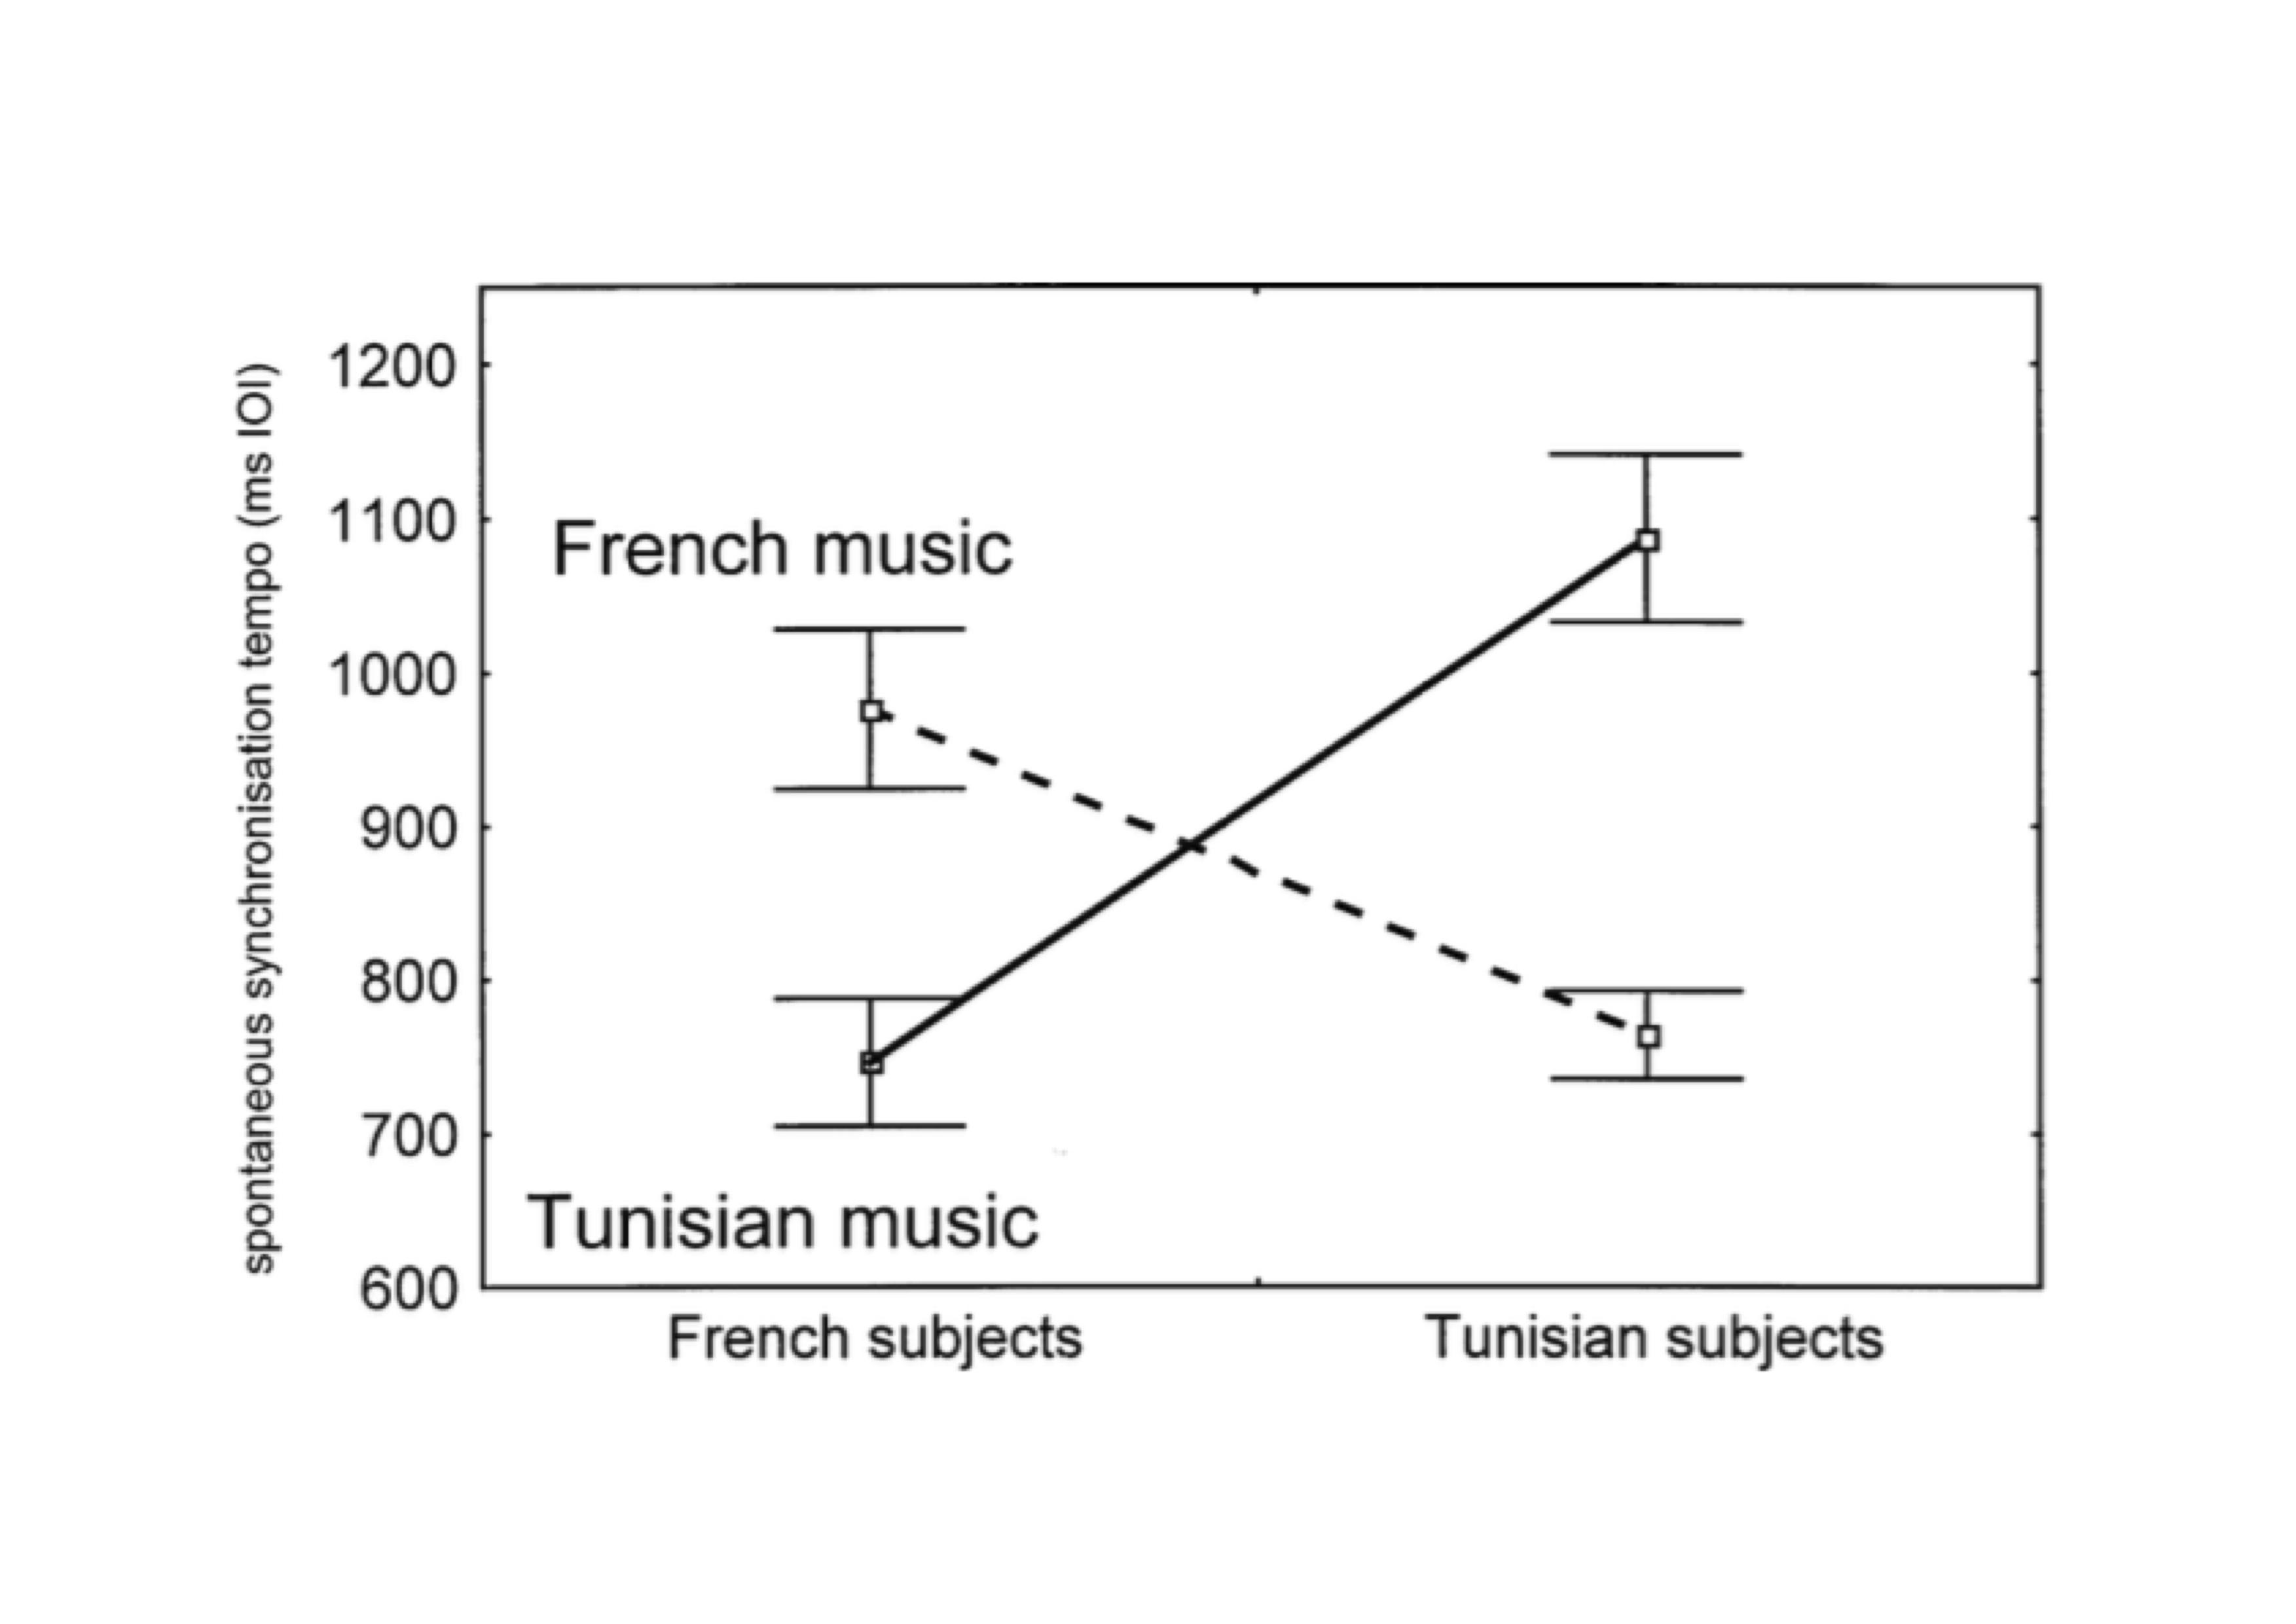
\includegraphics{figures/DrakeBenElHeni2003Fig2} 

}

\caption{Average time interval between taps (IOI, in ms) for two groups of listeners and two types of music (from Drake and Ben El Heni, 2003, Fig.2).}\label{fig:drakebenelheni2003fig2}
\end{figure}

\begin{quote}
These results show that there is no difference between both groups (French vs.~Tunisian listeners; both groups have the same IOI on average), and that there is also no difference between both types of music (French vs.~Tunisian music; both types of music result in the same IOI on average). Does this mean that the two independent variables have no effect at all? They absolutely do: it turned out that French listeners produced longer IOIs between taps when listening to French music, while, on the other hand, Tunisian listeners produced longer IOIs when listening to Tunisian music. Thus, all listeners produced longer IOIs when listening to a type of music they knew, and shorter IOIs when listening to a type of music they did not know. \citet{Drake03} conclude that listeners are better able to recognize and understand musical structure in music from their own musical culture compared to music from another culture. This pattern is a classic crossover interaction effect, in which one independent variable's effect is exactly opposite in the various conditions defined by the other independent variable.
\end{quote}

\begin{center}\rule{0.5\linewidth}{0.5pt}\end{center}

If it turns out that there is an interaction effect, we cannot sensibly interpret any main effects. This was already illustrated in example 6.5: we cannot conclude that there is no difference between the types of music. However, the size (and direction) of the difference depends on the other independent variable(s), in this case, group/nationality of listeners. Many studies are specifically aimed at demonstrating interaction effects: it is not main effects that are the topic of research, but their interaction, precisely as in example 6.5 above.

It is difficult to schematize a factorial research design, because it features multiple independent variables (with multiple levels each). We could schematically represent these by indexing the manipulation, which was previously shown simply as \texttt{X}. The first index (subscript) indicates the level for the first independent variable or factor, while the second index indicates the second factor's level. Following this system, we can schematize the design from example 6.5 as follows:

Als er een interactie-effect blijkt op te treden, dan is het zinloos om
een eventueel hoofdeffect te interpreteren. Dat werd al geïllustreerd in
Voorbeeld 6.5 hierboven: we kunnen niet concluderen dat er géén
verschil is tussen de muzieksoorten. Maar de grootte (en richting) van
het verschil is afhankelijk van de andere onafhankelijke variabele(n),

\begin{verbatim}
  R    X_{1,1}   O1
  R    X_{1,2}   O2
  R    X_{2,1}   O3
  R    X_{2,2}   O4
\end{verbatim}

Combining many factors into one big factorial design may often seem seductive: why not investigate how all these factors interact with one another? However, the most sensible option is not to do this, and, instead, limit the number of factors. Firstly, as we will see later, the number of observation has to keep up with the number of possible combinations of factors. Adding more factors means that many more participants (or other units) are needed. Secondly, it is more difficult to guarantee that all combinations of factors are perfectly comparable \citep[p.266]{SCC02}: may we reasonably compare Tunisian participants listening to Tunisian music in Tunisian with French participants listening to French music in France? The more combinations of factors are featured in the study, the trickier it becomes to ensure that these combinations are comparable. Thirdly, interactions are notoriously difficult to interpret, which also becomes trickier as interactions become more complex and span a greater number of factors. For all of these reasons, it is better to study the effects of multiple factors in separate individual studies \citep{Quene10}.

We will come back later to the analysis and interpretation of data from factorial experimental designs (Chapter \ref{ch:anova}).
In the meantime, we will concentrate on designs that have just one independent variable.

\hypertarget{sec:within-subject-designs}{%
\section{Within-subject designs}\label{sec:within-subject-designs}}

At the outset of the chapter, we spoke about manipulating an independent variable either between or within subjects ((§\ref{sec:betweenwithinparticipants}). In most designs discussed above, a separate group was formed for each value of the independent variable(s); we call this a between subjects design. The independent variable's value differs between participants.

However, some independent variables may also be manipulated within participants. In such cases, we take repeated measures for (within) the same participants from the same group, switching out different conditions of the independent variable. In the example below, the independent variable, `language' (native or non-native), is varied within participants. We call this a within subjects design.

\begin{center}\rule{0.5\linewidth}{0.5pt}\end{center}

\begin{quote}
\emph{Example 6.6}: \citet{JGSH13} investigated the fluency of participants' speech in their native language (Turkish) and in a non-native language (Dutch). The participants first performed a number of speech production tasks in their native language, a few weeks after which they did the same for Dutch. One of the dependent variables was the number of filled pauses (e.g., \emph{uh, uhm}) per second of speech: the greater the prevalence of pauses, the lesser the degree of fluency. As we might expect, the speakers did turn out to produce more pauses (i.e., speak less fluently) in the non-native language compared to their native language. However, one of the goals of this study was to investigate to which extent we may trace back individual fluency differences in the non-native language to individual fluency differences in the native language. These two measurements turned out to be highly correlated (\(r = 0.73\); see Chapter \ref{ch:correlation} for more on this). Speakers that have many pauses in the non-native language also have many pauses in their native language. The researchers argue that we must take this correlation into account when teaching and testing speaking ability in a non-native language.
\end{quote}

\begin{center}\rule{0.5\linewidth}{0.5pt}\end{center}

The research design described here can be schematized as follows:

\begin{verbatim}
   X1   O1   X2   O2
\end{verbatim}

Despite the many threats it poses to internal validity (including history, maturation, guiding influence of pretests), such a design is often useful. In the example above, it is essential that it is the \emph{same} participants that carry out speaking tasks in both languages (conditions) -- no other method will be adequate for answering the research questions.

\hypertarget{designing-a-study}{%
\section{Designing a study}\label{designing-a-study}}

A researcher who intends to carry out a study has to settle on a way of collecting data: they have to choose a particular design for their study. Sometimes, a standard designed may be chosen, for instance, one of the designs discussed above. In other cases, the researcher will have to devise their own design. Naturally, the design chosen should fit well with the research question \citep{Levin99}, and it should exclude as many disruptive, potentially validity-threatening variables as possible. Designing a study is a skill that researchers hone with practice. In the example below, we will try to show to you which reasoning and arguments play a role in developing a design for a study.

Suppose that we would like to investigate whether the way in which test questions are asked, as open vs.~closed questions, influences students' scores on the relevant test. If we use a simple design, we will first administer a test with open questions to a group of respondents, and then, a comparable test with closed questions to the same respondents. If the resulting scores are sufficiently correlated, we conclude that both tests measure the same thing, and that performance on the test is not significantly influenced by the way questions are asked. This design can be schematized as follows:

\begin{verbatim}
   Open   O1   Closed   O2
\end{verbatim}

However, this research design does have various weaknesses. Firstly, it is not prudent to first administer all open question tests at the first time point, and leave all closed question tests for the second time point. This is because performance on the second test will always be influenced by effects of ordering (transfer effects): respondents remember and, thus, learn something from the first measurement. However, this transfer always works in one direction, which means that we expect relatively higher performance on the test with closed questions (at the second time point). Because of this, it is better to randomly distribute the open question and close question tests between the first and second time point.

Secondly, all respondents might have been influenced by any events that took place between the two time points (history), for instance, by some instruction relevant to the test's subject matter. Because there is no control group, we cannot take this type of effect into account.

A third problem lies in the way in which the reasoning from findings to conclusions is constructed. For the current example, we defined this reasoning as follows: if scores on both tests are sufficiently correlated, both tests measure the same thing. If you stop and think about it, you might agree with us that this is a strange bit of reasoning. The underlying research question really seems to be whether the correlation between performance on different tests with different types of questions is the same as the correlation between performance on different tests with the same types of questions, since we do assume that the latter group of tests measure the same thing. This, in itself, defines a control group: respondents who, at both points in time, write tests with the same types of questions. Just to be sure, let us add not one, but two control groups: one with open questions at both time points, and one with closed questions at both time points.

By doing this, we have improved the design in at least two ways: (1) tests are randomized between times of measurement, and (2) relevant control groups have been added. At this point, we may schematize our design as follows:

\begin{verbatim}
       Exp. group 1       Open    O1   Closed   O2
       Exp. group 2      Closed   O3    Open    O4
      Control group 1     Open    O5    Open    O6
      Control group 2    Closed   O7   Closed   O8
\end{verbatim}

For all four groups, we may now determine the correlation between their performance at the first and the second time point. We can subsequently compare these correlation results between the four groups, and use this to answer the research question. This example shows us that the conclusions that can be draw from research results are directly dependent on the design that was chosen \citep{Levin99}. In the first design, a low correlation would lead to a conclusion that the two types of testing investigated do \emph{not} test for the same intellectual skills in our respondents. However, in the second design, the same low correlation in the first group (experimental group 1) does not have to lead to the same conclusion! This is because the conclusion also depends on the degree of correlation that was found in the other groups.

\hypertarget{in-conclusion}{%
\section{In conclusion}\label{in-conclusion}}

Despite all the books, manuals, websites, and other instructional materials that are available, it is still much too often that we encounter studies with methodological problems in their research questions, operationalization, design, drawing of samples, and/or data collection. Not only do these problems cause a waste of time, money, and energy, but they also yield knowledge that is less reliable, valid, and robust than would otherwise have been possible. The following checklist for good research practice (partly taken from \url{https://www.linkedin.com/groups/4292855/4292855-6093149378770464768}) may preempt many problems during a study's later stages.

\begin{enumerate}
\def\labelenumi{\arabic{enumi}.}
\item
  Give your research questions plenty of thought, and formulate them fully into the smallest detail. If the questions have not been formulated clearly, or if there are many sub-questions, keep working on the questions.
\item
  Arrange the research questions according to their priority. This will help in making good choices regarding design, sampling, operationalization, etc.
\item
  Think long and hard about your study's design. According to an informal rule of thumb, each hour spent thinking about your study's design will save you 10 hours of additional data analysis and interpretation in the future. Put differently: spending an hour less on thinking about your design will cost you 10 hours of work down the road.
\item
  Think of various alternative designs for your study, and think about each possible design option's advantages and disadvantages.
\item
  Imagine the future: you have completed your research project, analysed your data, and written your report or thesis. Which message would you like to impart upon the readers of your report? How does your study's design contribute to this message? What might you change in your design to make this message even clearer? Think of the direction you would like to take, not just of where you are now.
\item
  Write a research plan in which you describe the various methodological aspects of your study. Explain the details of and the reasoning behind your research questions, design, sample, method of measurement, data collection, instruments of measurement (e.g., questionnaire, software), other requirements (e.g., laboratory environment, transportation), and statistical processing. You will be able to reuse parts of this research plan in your report. When writing your plan, make sure to include a schedule: when will which milestone be reached?
\item
  Write out what statistical analyses you will use on your data before your actually start collecting any data. Again, be as explicit as possible (using a script, step-by-step plan, or similar). Make up a miniature collection of fake observations, or real observations from the pilot phase of your study, and analyse these data as if this were your definitive collection of data. Make adjustments to your research plan as needed.
\item
  Once you are collecting data, do \emph{not} make any changes to your research plan. Keep to this plan and the schedule you made. Analyse your data in the way specified in the (previously adjusted) research plan. Do discuss in your report any problems that arose during the study. If serious problems occur, halt your project, and consider starting anew with an improved version of your study.
\end{enumerate}

  \bibliography{book.bib,packages.bib,hhmhto.bib,pandoc.bib}

\end{document}
